\documentclass[a4paper, 12pt]{article}
\usepackage[T1]{fontenc}
\usepackage{lmodern}
\usepackage{color}
\usepackage{amsfonts}
\usepackage{epstopdf}
\usepackage{matlab}
%\documentclass{book}
\usepackage{blindtext}
\usepackage{hyperref}
\usepackage[brazil]{babel}
\usepackage{amssymb}
\usepackage[utf8]{inputenc}
\usepackage{amsmath}
\usepackage{indentfirst}
\usepackage{graphicx}
\usepackage{multicol,lipsum}
\usepackage[a4paper,
top=3cm, left=3cm, bottom=3cm, right=3cm]{geometry}
\usepackage{setspace}
\usepackage{multirow}
\usepackage{float}
\usepackage[table]{xcolor}
%\usepackage{pdflscape}
\usepackage[DIV=15]{typearea}
\usepackage[nottoc]{tocbibind}
\usepackage[sort,numbers]{natbib}
%\usepackage{cite}
\usepackage{matlab}


\documentclass[letterpaper]{article}
% bib pack %%%%%%%%%%%%%%%%%%%%%%%%%%%%%%%%%%%%%%%%%%%%%%%%%%%%%%%%%%%%%%%%%%%%%
\usepackage[utf8]{inputenc}
\usepackage{geometry}
    \geometry{left=3cm,right=2cm,top=2cm,bottom=2cm}
%
\usepackage[spanish]{babel}
%
\usepackage[fixlanguage]{babelbib}
    \bibliographystyle{babunsrt}
%
\usepackage{url}

\begin{document}
%\maketitle

\begin{titlepage}
	\begin{center}
		

\vspace{10pt}
%\begin{figure}[!ht]
%\centering
%
\includegraphics{puc-rio-logo.png}

%\end{figure}
\begin{figure}[!ht]
\centering

\includegraphics{images/puc-rio-logo.png}
\end{figure}
\huge{Laboratório de Controles e Servomecanismos}
        \vspace{70pt}
        
		\textbf{ENG1418}
		\textbf{\large{\\ }}
		
		\vspace{30pt}
		\textbf{\small{\\Trabalho 07}}
		\vspace{75pt}
		
	\end{center}
	
	\begin{flushleft}
		\begin{tabbing}
			Aluno(a)\qquad\qquad\=\>Gabriel Mota Botelho - 1620628 \\ \>Paloma Fernanda Loureiro Sette - 1621595\\
			
			Professor(a)\>Vivian Suzano Medeiros\\
	\end{tabbing}
		  
	\end{flushleft}
	\begin{center}
		%\vspace{\fill}
		\vspace{90pt}
		Rio de Janeiro, 07 de Julho de 2022
	\end{center}
\end{titlepage}
%%%%%%%%%%%%%%%%%%%%%%%%%%%%%%%%%%%%%%%%%%%%%%%%%%%%%%%%%%%
\newpage
\tableofcontents
\thispagestyle{empty}

\newpage
\pagenumbering{arabic}

\newpage

%\newcommand{\listequationsname}{Lista de Equações}
%\newlistof{myequations}{equ}{\listequationsname}
%\newcommand{\myequations}[1]{%
%\addcontentsline{equ}{myequations}{\protect\numberline{\theequation}#1}\par}

%\listofmyequations


\newpage
\listoffigures

\pagebreak
%%%%%%%%%%%%%%%%%%%%%%%%%%%%%%%%%%%%%%%%

\section{Introdução}
O objetivo deste trabalho é consolidar os conhecimentos de ações de controle estudados na disciplina ENG1417 – Controles e Servomecanismos. Ele é dividido em duas partes. A primeira, uma preparação, utiliza materiais educacionais existentes no Maxwell para rever e simular ações de controle. A segunda é o experimento no Laboratório Remoto da UNED.

\section{Realização do Trabalho}
A UNED – Universidad Nacional de Educación a Distancia (\url{https://www.uned.es/universidad/inicio.html}) é uma universidade espanhola, com sede em Madrid cuja missão é oferecer cursos de graduação, pósgraduação e extensão na modalidade a distância. Entre seus inúmeros projetos, está o UNILabs – \textit{University Network of Interactive Labs} (\url{https://unilabs.dia.uned.es/}), que podem ser simulados por software ou com acesso a hardware.\\

No UNILabs está disponível dois laboratórios remotos de um servomotor, que serão utilizados para a realização desse trabalho. Um laboratório virtual, baseado na simulação do sistema, e um laboratório real, que mostra um motor físico real.\\

Laboratório virtual: \url{https://unilabs.dia.uned.es/mod/ejsapp/view.php?id=2416} \\
Laboratório remoto: \url{ttps://unilabs.dia.uned.es/mod/ejsapp/view.php?id=2417}. 

\section{Roteiro}
Considere o sistema apresentado na figura a seguir, um motor de corrente contínua controlado pela corrente de armadura. Uma tensão de entrada ua é aplicada no circuito de armadura do motor, fazendo com que o eixo gire a uma velocidade angular proporcional a tensão induzida na armadura. O coeficiente de atrito nos mancais é representado por bm e gera uma força de resistência proporcional a velocidade angular do motor.

\begin{figure}[H]
\centering
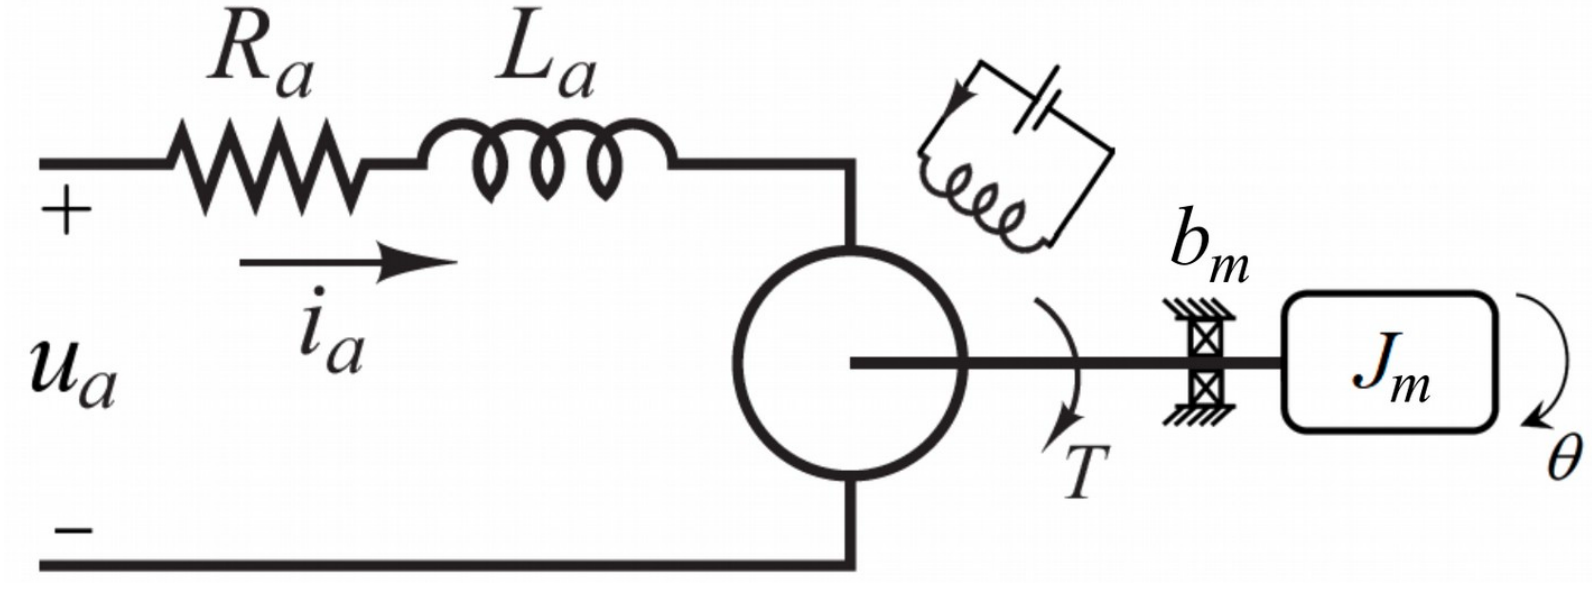
\includegraphics[scale = 0.4]{images/sistema-motor.png}
\label{filtro1}
\caption{Motor C.C. controlado pela corrente de armadura}
\end{figure}

A tabela a seguir descreve os parâmetros deste sistema:

\begin{table}[H]
\resizebox{\textwidth}{!}{%
\begin{tabular}{|l|l|}
\hline
\textbf{Parâmetros} & \textbf{Símbolo} \\ \hline
Resistência de armadura & $R_a$   \\ \hline
Indutância da armadura & $L_a$  \\ \hline
Constante de torque & $K_t$  \\ \hline
Constante de fcem & $K_e$ \\ \hline
Momento de inércia do motor & $J_m$ \\ \hline
Atrito linear no movimento do motor & $b_m$  \\ \hline
\end{tabular}%
}
\caption{Equivalentes Elétricos e Térmicos}
\end{table}

As equações de movimento que descrevem esse sistema são dadas por:

\begin{equation}
    \begin{cases}
    L_a\frac{di_a(t)}{dt}=u_a(t)-R_ai_a(t)-K_e\frac{d\theta(t)}{dt} \\
    J_m\frac{d^2\theta(t)}{dt^2} = K_ti_a(t)-b_m\frac{d\theta(t)}{dt}
    \end{cases}
\end{equation}

Assumindo que a indutância da armadura é desprezível ($L_a \approx 0H$), as equações acima podem ser simplificadas para:

\begin{equation}
    J_m\frac{d^2\theta(t)}{dt^2} = \frac{K_t}{R_a}u_a(t)-(b_m+\frac{K_tK_e}{R_a})\frac{d^2\theta(t)}{dt^2} = Ku_a(t)-B\frac{d\theta(t)}{dt}
\end{equation}

A função de transferência correspondente é:

\begin{equation}
    \frac{\theta(s)}{U_a(s)} = \frac{K}{s(J_ms+B)}
\end{equation}

Assumindo que a saída do sistema é a velocidade angular, a função de transferência é:

\begin{equation}
    \frac{\omega(s)}{U_a(s)} = \frac{K}{J_ms+B}=\frac{\frac{K}{B}}{\frac{J_m}{B}+1}=\frac{K_\omega}{\tau s+1}
\end{equation}

Logo, é possível caracterizar o comportamento do sistema a partir da identificação dos parâmetros $K_\omega$ e $\tau$. Para identificar esses parâmetros é possível usar a resposta do sistema a um degrau unitário.

\begin{figure}[H]
\centering
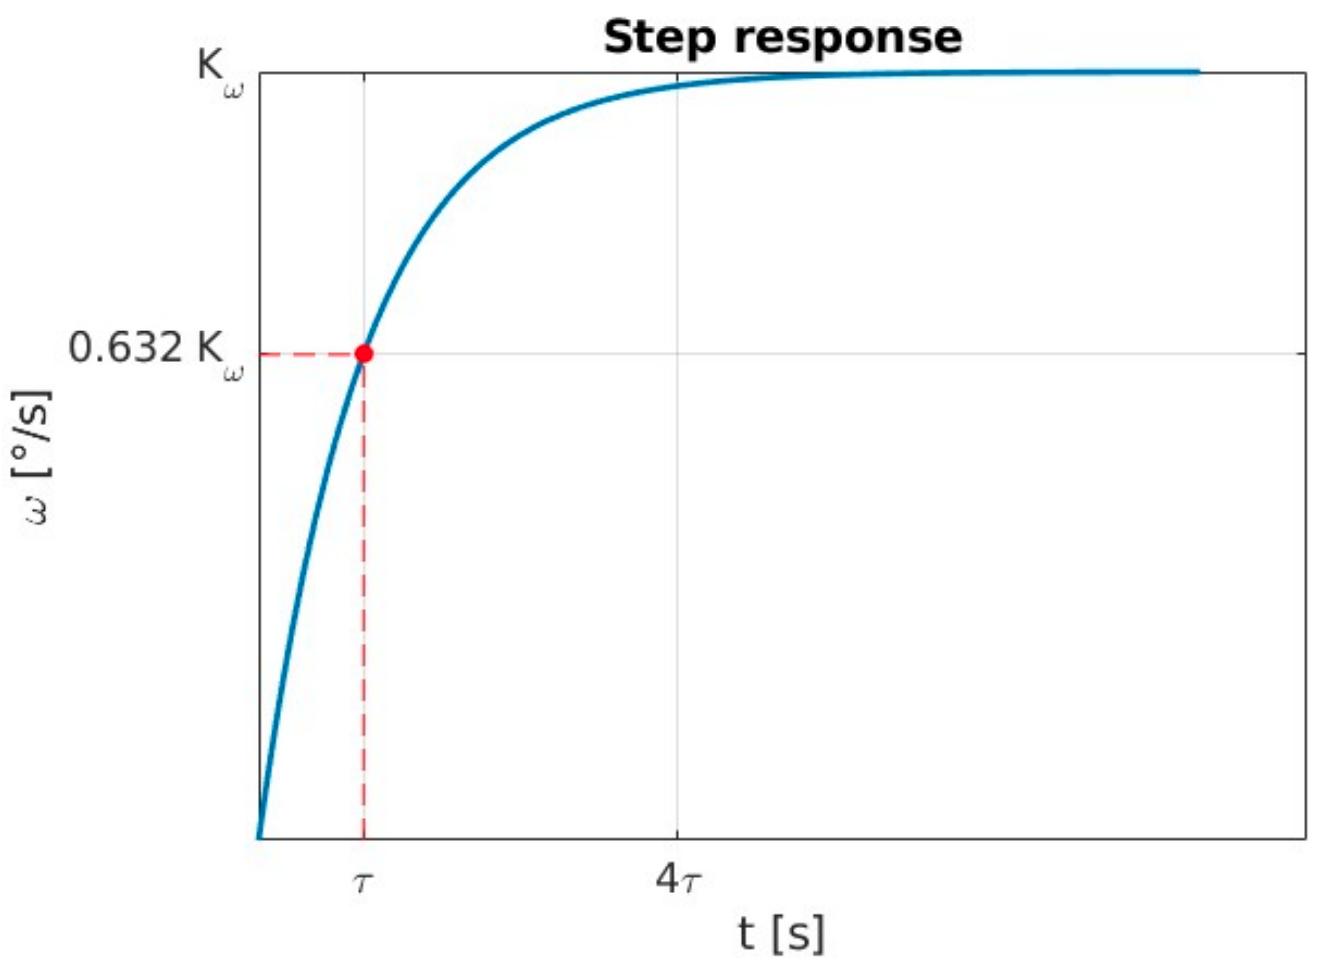
\includegraphics[scale = 0.6]{images/step-response-abordagem.png}
\label{filtro1}
\caption{Gráfico de resposta ao degrau unitário - Abordagem}
\end{figure}

O valor em regime permanente da resposta é $K_\omega$ e o tempo onde a resposta atinge 63.2\% do valor final é a constante de tempo $\tau$.
Com base nisso, siga os seguintes passos usando o Laboratório Virtual da UNED (\url{https://unilabs.dia.uned.es/mod/ejsapp/view.php?id=2416}) para fazer a identificação dos parâmetros do motor utilizado no laboratório remoto.

\subsection{Tarefa 1 - Identificação dos parâmetros do motor}
\subsubsection{Determinando o ganho $K_\omega$}
\paragraph{(a) Reinicie o sistema (pressione o botão Reset)} :\\

Sistema reiniciado.

\paragraph{(b) Envie uma tensão de 1 V para o motor e anote a leitura de velocidade.} : \\

Como podemos observar na imagem abaixo, ao selecionar o valor de 1 V para o servomotor, foi obtido 5.75 para a velocidade (\textit{speed})
\begin{figure}[H]
\centering
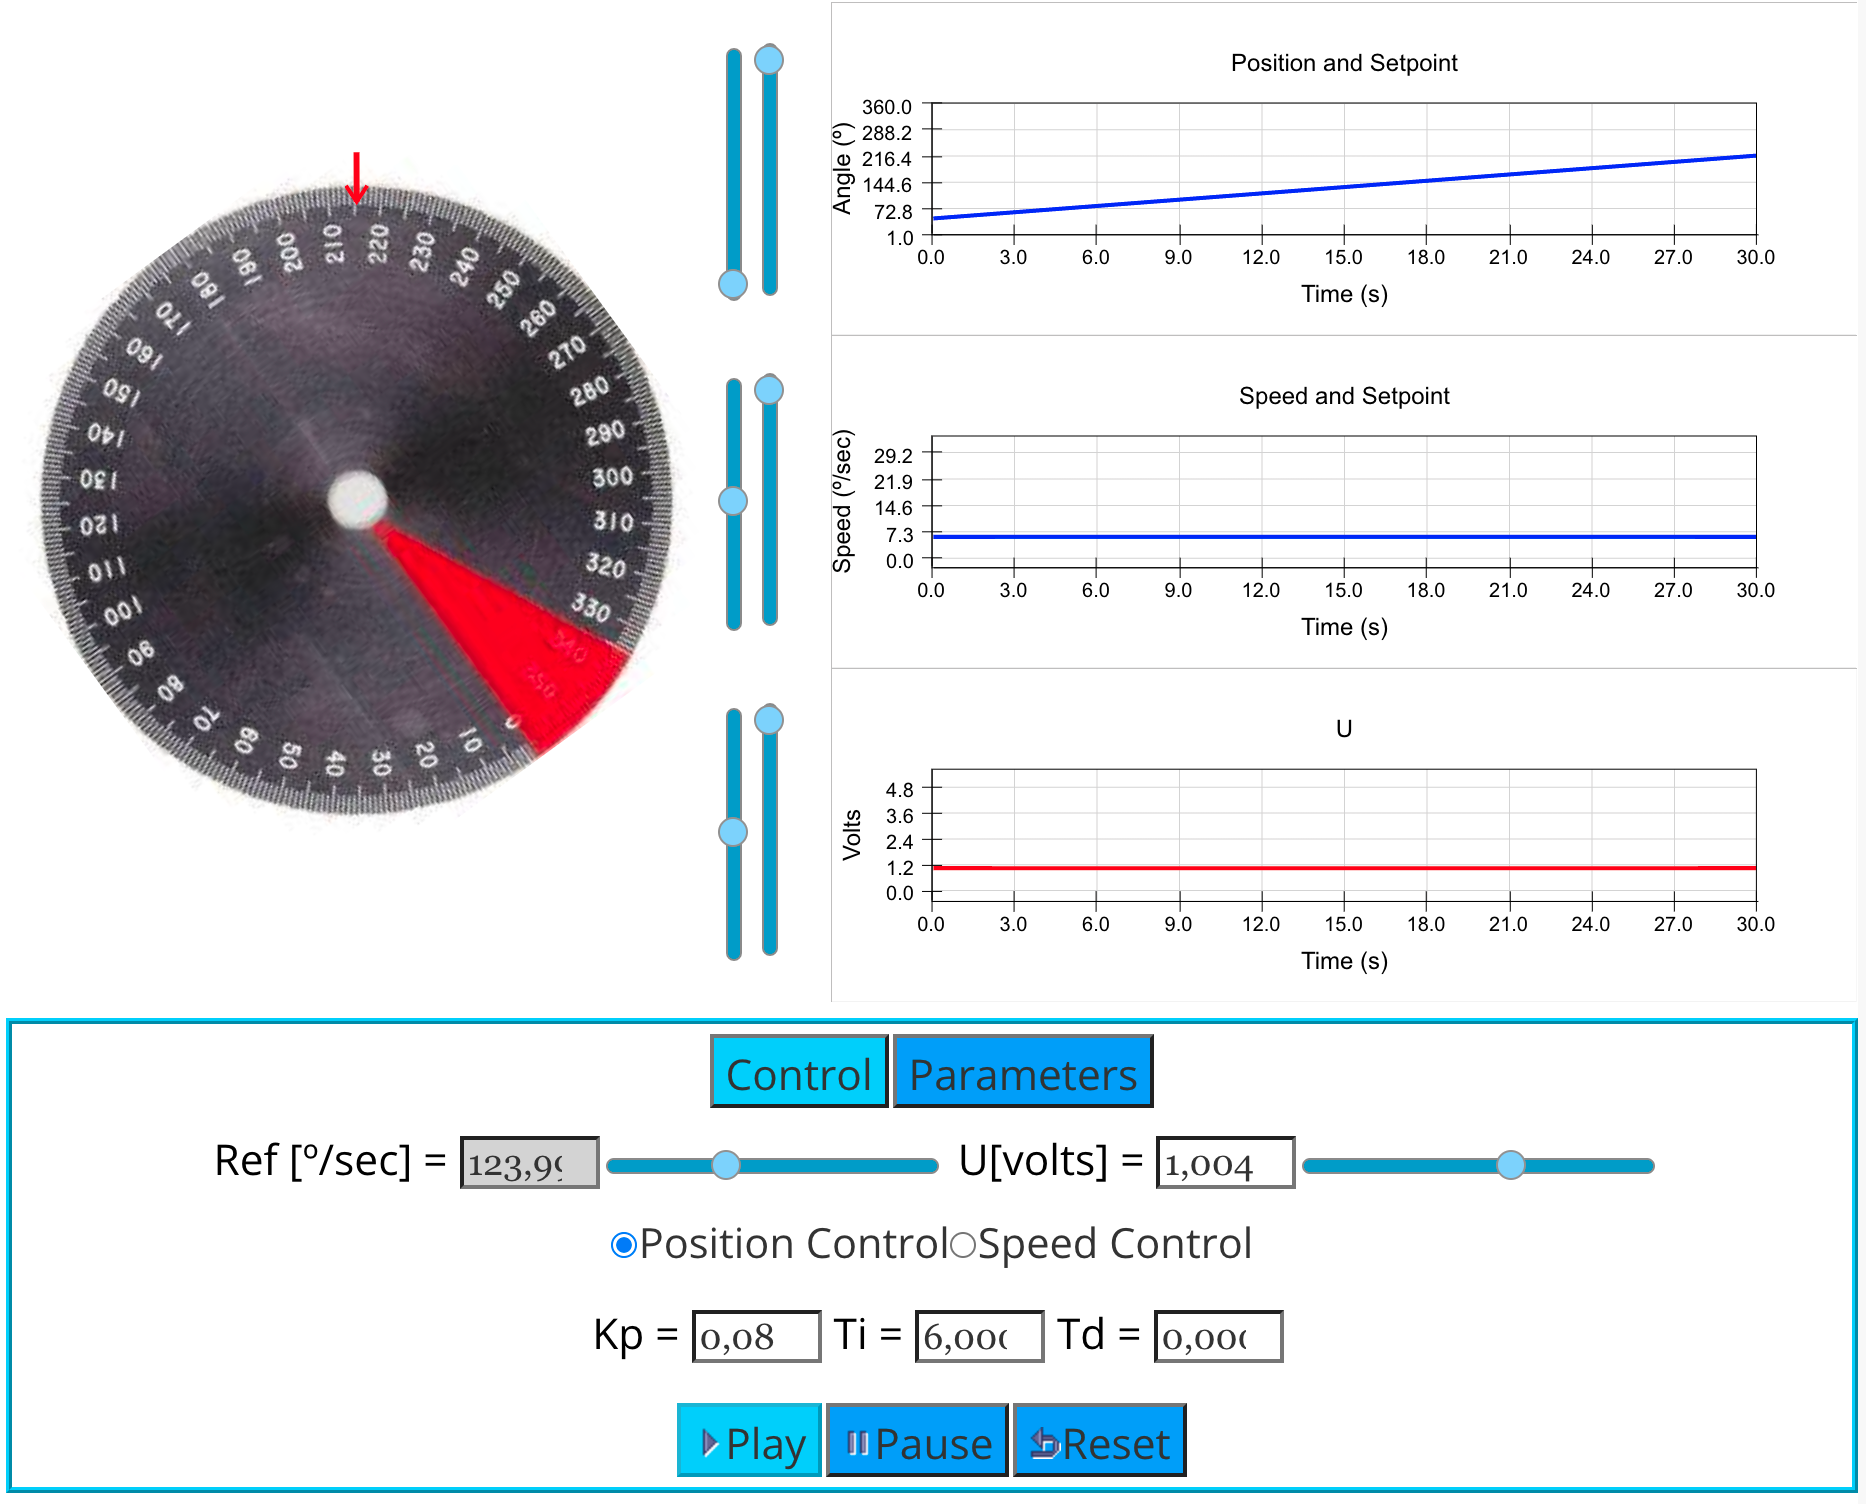
\includegraphics[scale = 0.5]{images/cap-1_uned_lab-virtual-tensao-motor.png}
\label{filtro1}
\caption{Laboratório Virtual da UNED - Selecionando 1V para o motor}
\end{figure}

\begin{figure}[H]
\centering
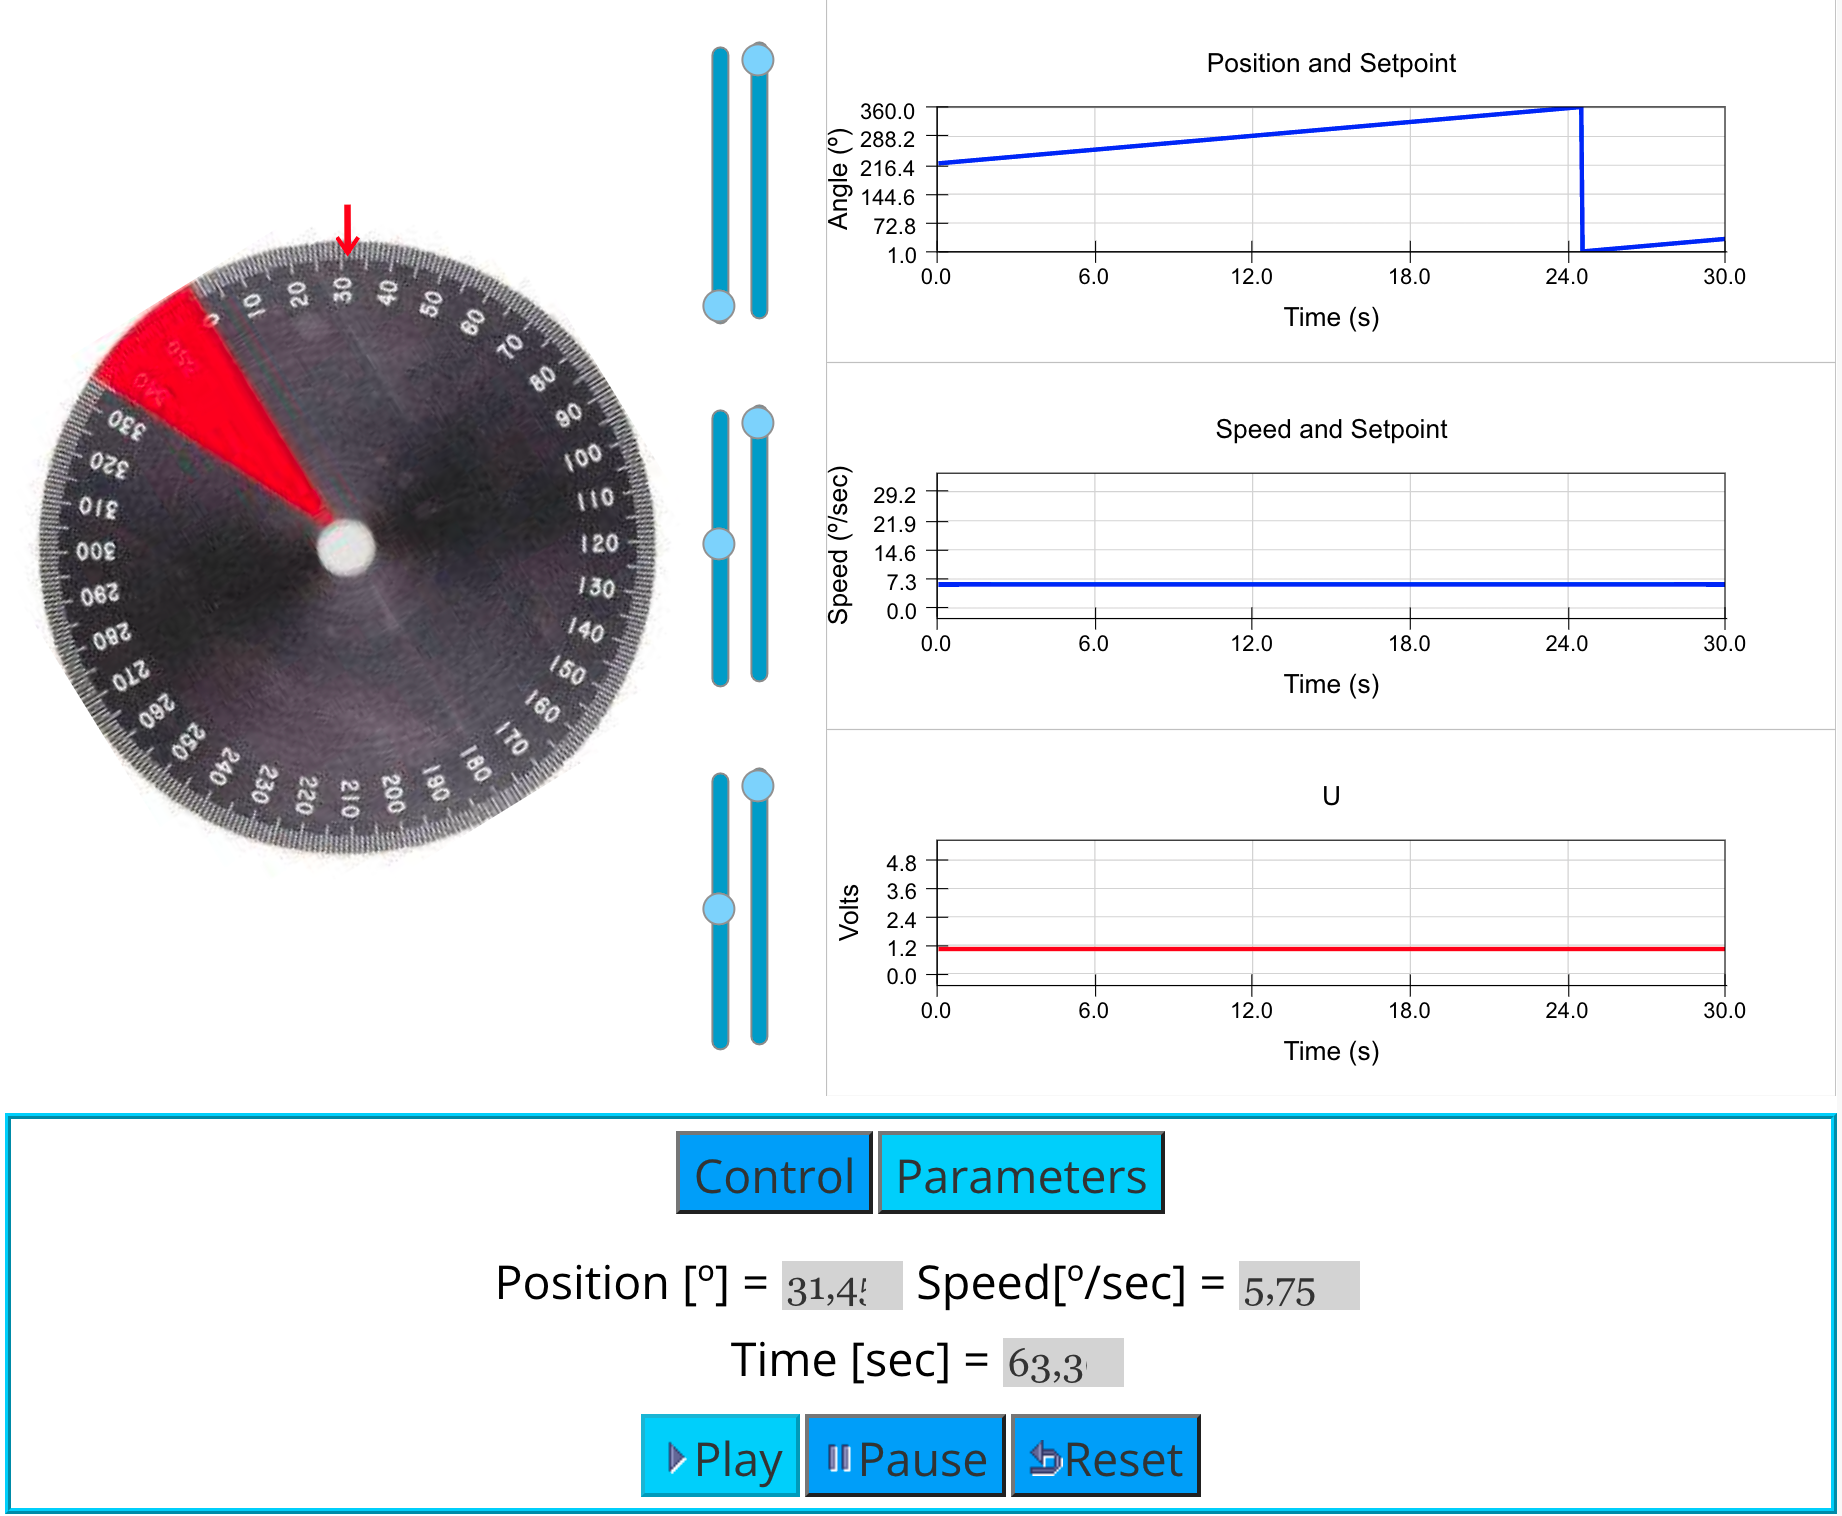
\includegraphics[scale = 0.5]{images/cap-1_uned_lab-virtual.png}
\label{filtro1}
\caption{Laboratório Virtual da UNED - Velocidade do motor}
\end{figure}

Velocidade = 5,75º/sec\\
\paragraph{(c) Repita as medições com incrementos de 0,5V na tensão do motor até 3V. }:\\

Nota: A inclinação da linha reta que melhor ajusta os pontos obtidos (tensão, velocidade) é o ganho da função de transferência.\\

\newpage
- \qquad\qquad\> Para 0,5V: 
\begin{figure}[H]
\centering
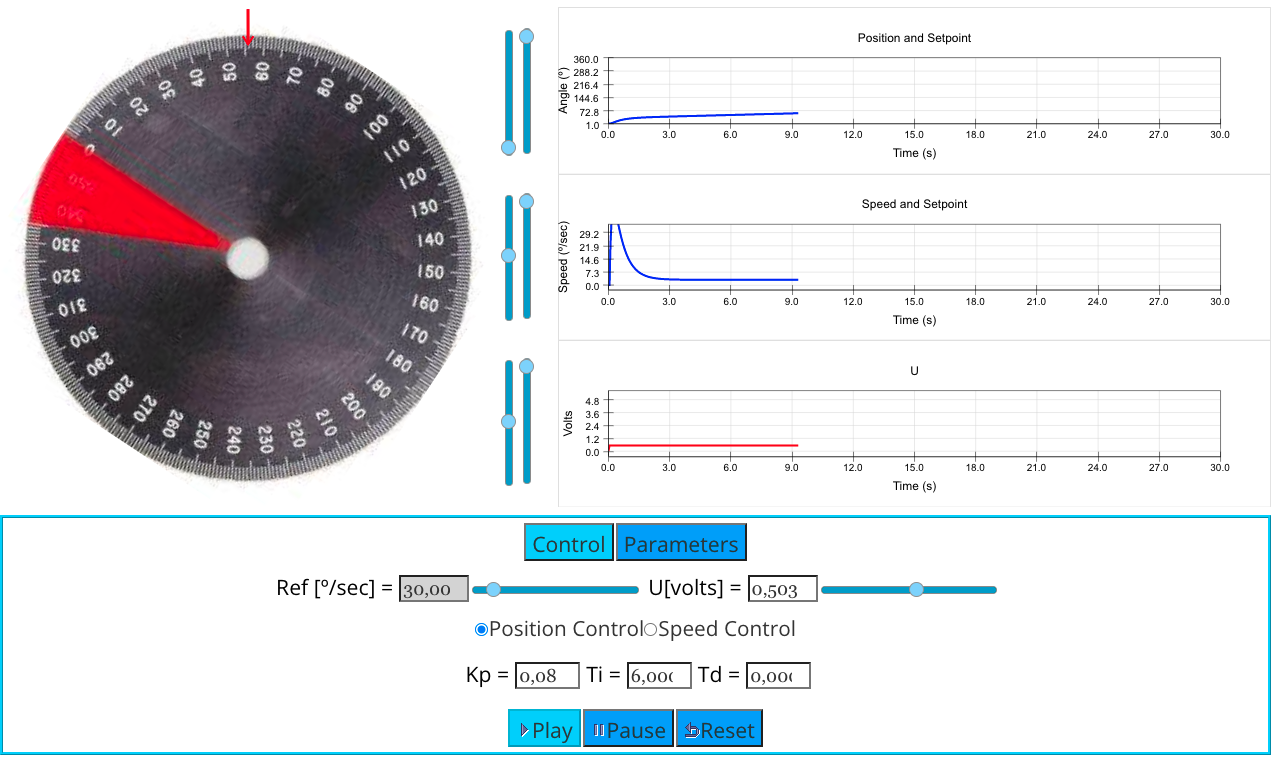
\includegraphics[scale = 0.35]{images/pt1-c-05.png}
\label{filtro1}
\caption{Medição a 0.5V - Controle}
\end{figure}

\begin{figure}[H]
\centering
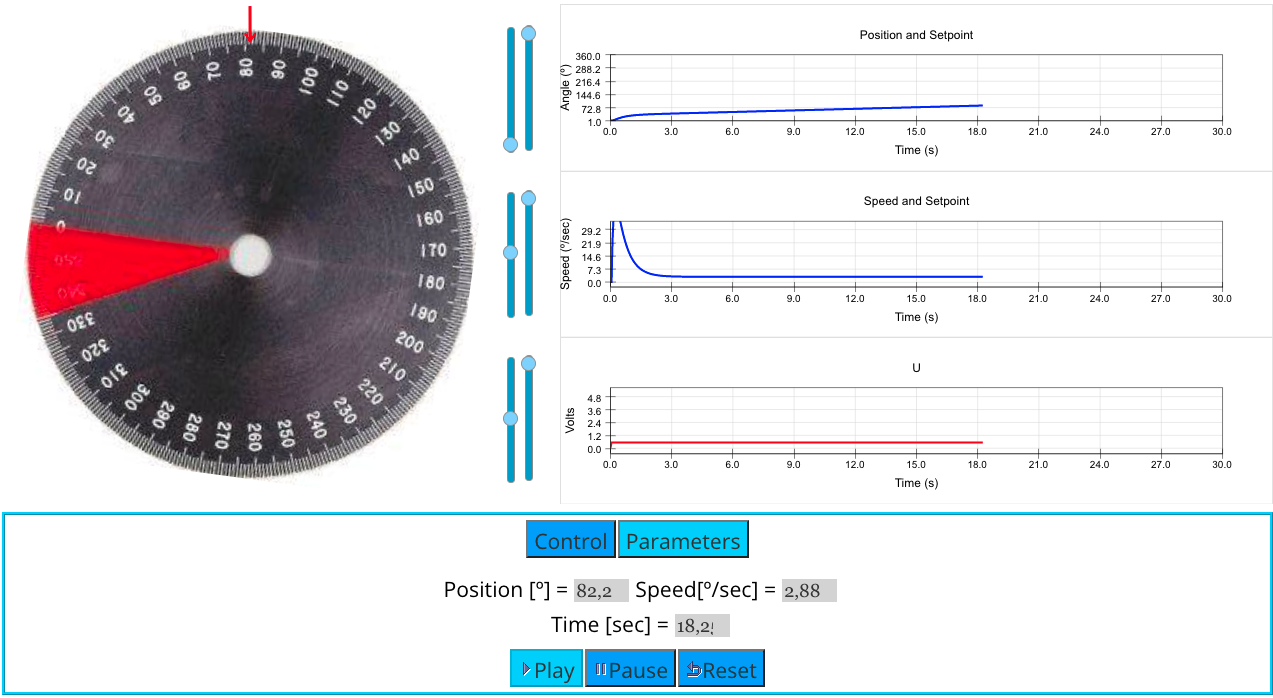
\includegraphics[scale = 0.35]{images/pt1-c-05-param.png}
\label{filtro1}
\caption{Medição a 0.5V - Parametros}
\end{figure}

Velocidade = 2,88º/sec\\\\

\newpage
- \qquad\qquad\> Para 1,0V: 
\begin{figure}[H]
\centering
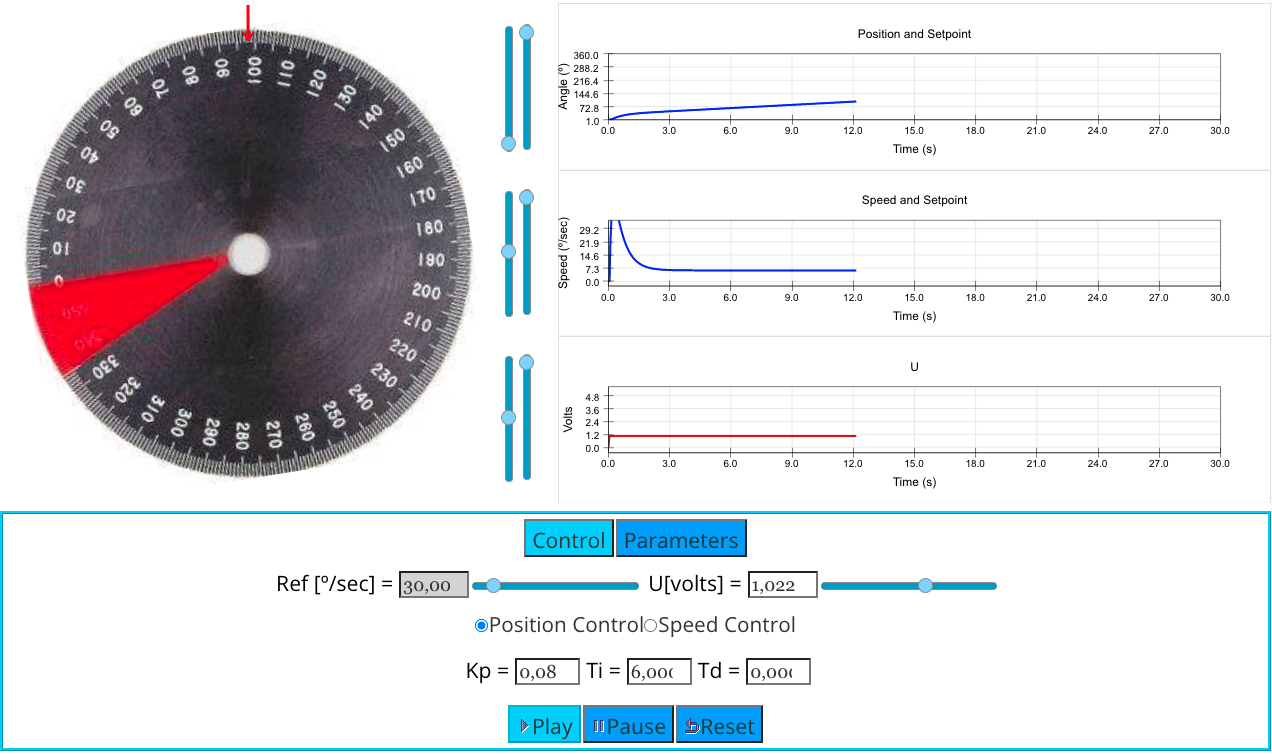
\includegraphics[scale = 0.35]{images/pt1-c-1-control.png}
\label{filtro1}
\caption{Medição a 1V - Controle}
\end{figure}

\begin{figure}[H]
\centering
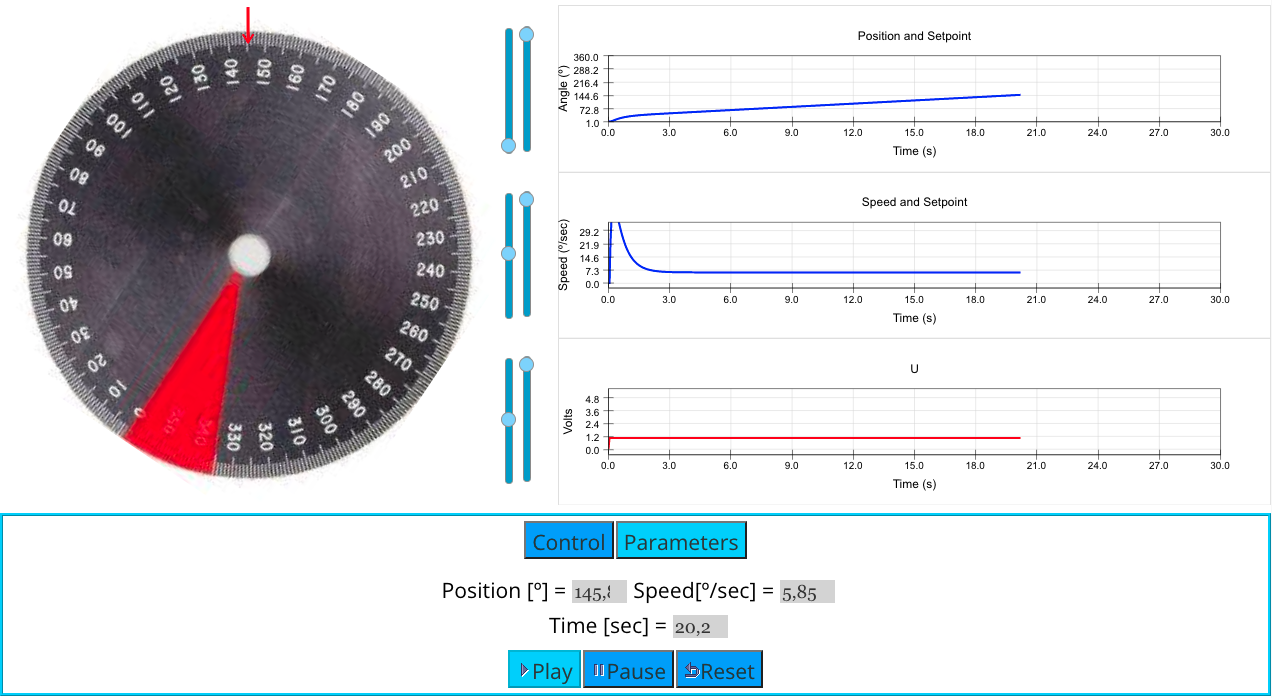
\includegraphics[scale = 0.35]{images/pt1-c-1-param.png}
\label{filtro1}
\caption{Medição a 1V - Parametros}
\end{figure}

Velocidade = 5,85º/sec\\\\


\newpage
- \qquad\qquad\> Para 1,5V: 
\begin{figure}[H]
\centering
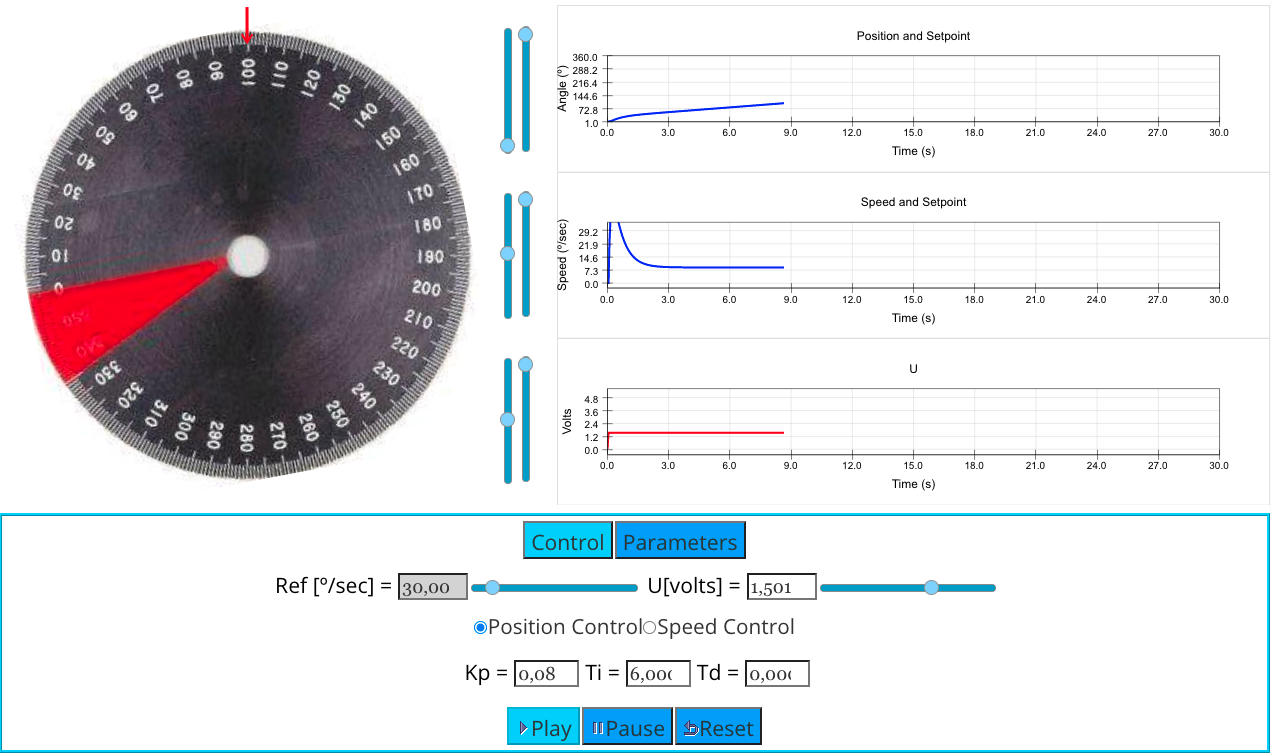
\includegraphics[scale = 0.35]{images/pt1-c-15-control.png}
\label{filtro1}
\caption{Medição a 1,5V - Controle}
\end{figure}

\begin{figure}[H]
\centering
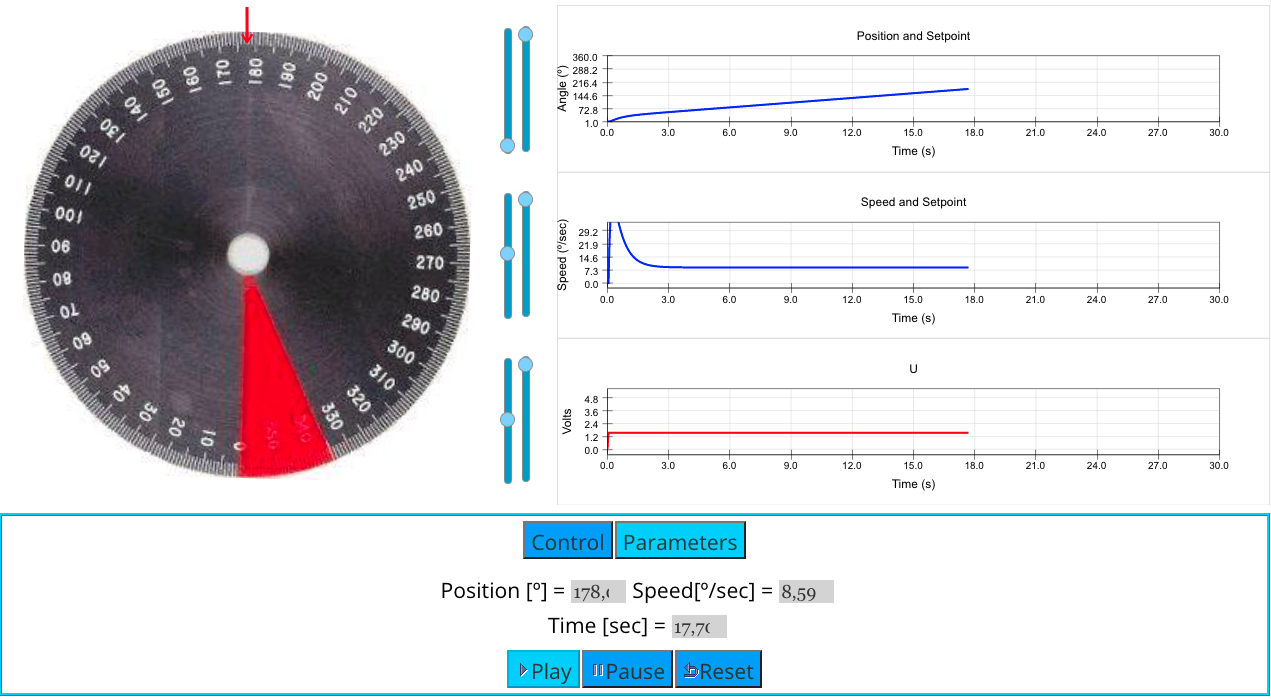
\includegraphics[scale = 0.35]{images/pt1-c-15-param.png}
\label{filtro1}
\caption{Medição a 1,5V - Parametros}
\end{figure}

Velocidade = 8,59º/sec\\\\


\newpage
- \qquad\qquad\> Para 2V: 
\begin{figure}[H]
\centering
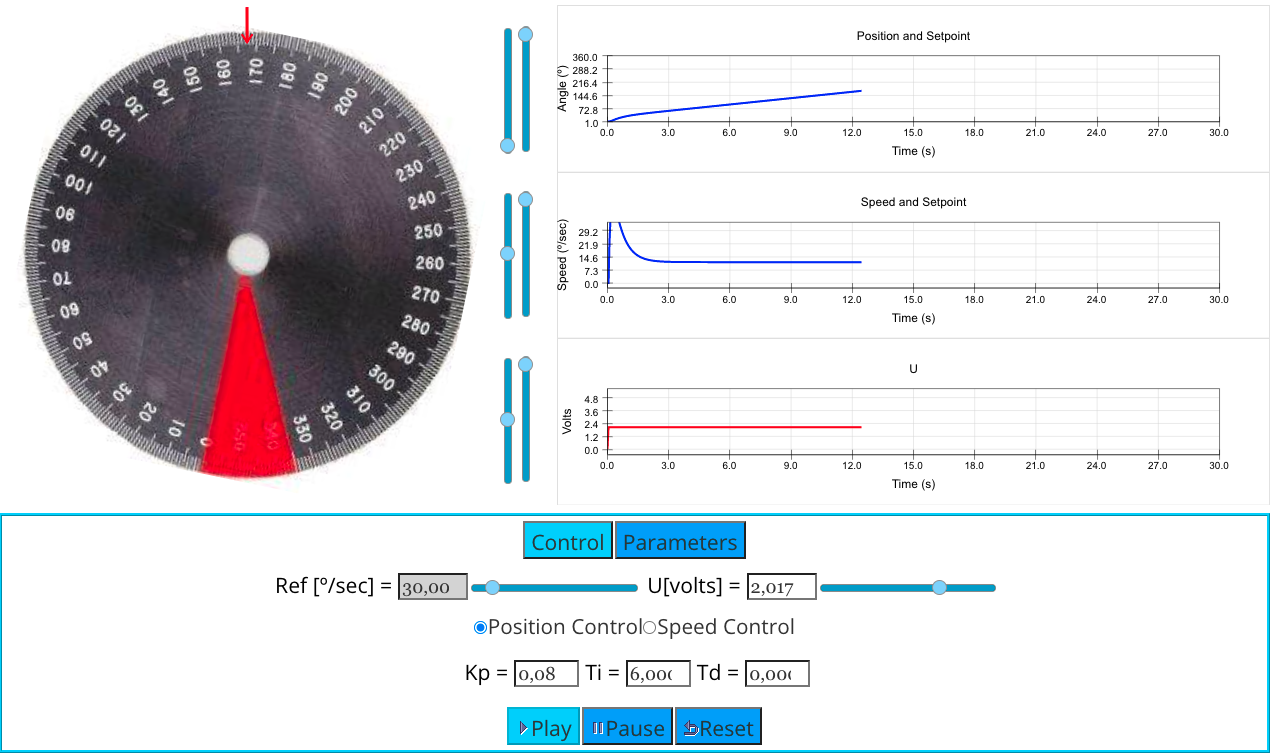
\includegraphics[scale = 0.35]{images/pt1-c-2-control.png}
\label{filtro1}
\caption{Medição a 2V - Controle}
\end{figure}

\begin{figure}[H]
\centering
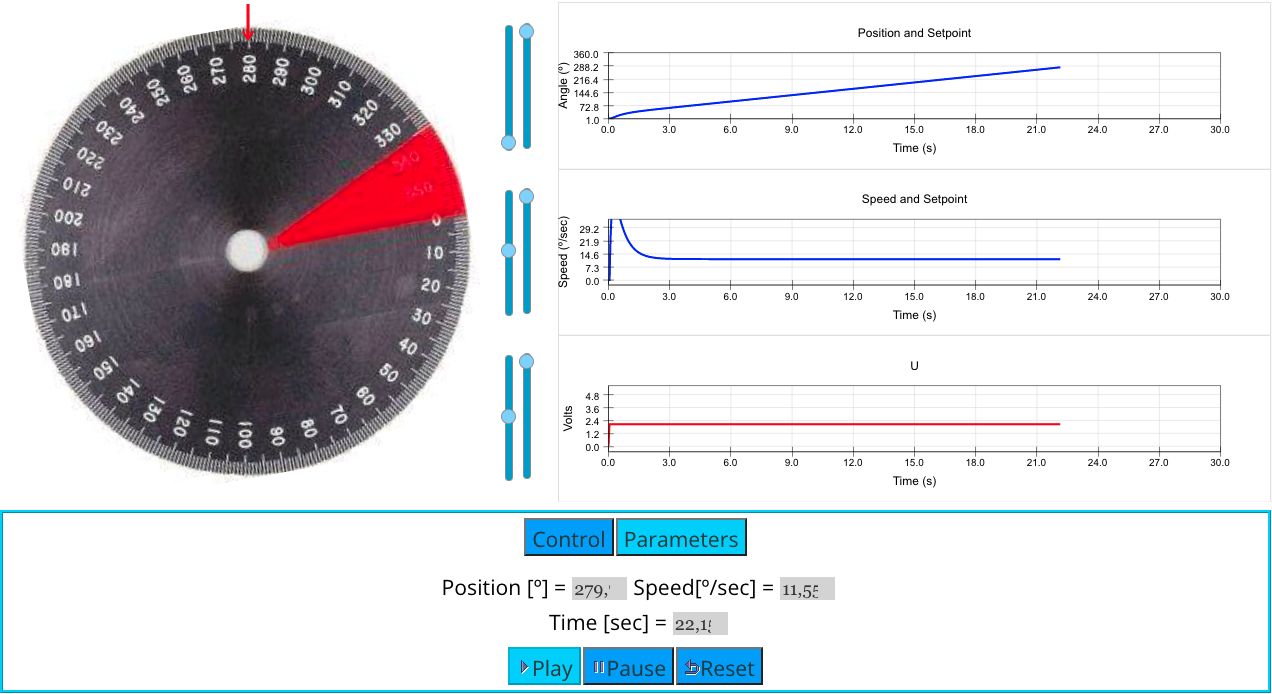
\includegraphics[scale = 0.35]{images/pt1-c-2-param.png}
\label{filtro1}
\caption{Medição a 2V - Parametros}
\end{figure}

Velocidade = 11,55º/sec\\\\


\newpage
- \qquad\qquad\> Para 2,5V: 
\begin{figure}[H]
\centering
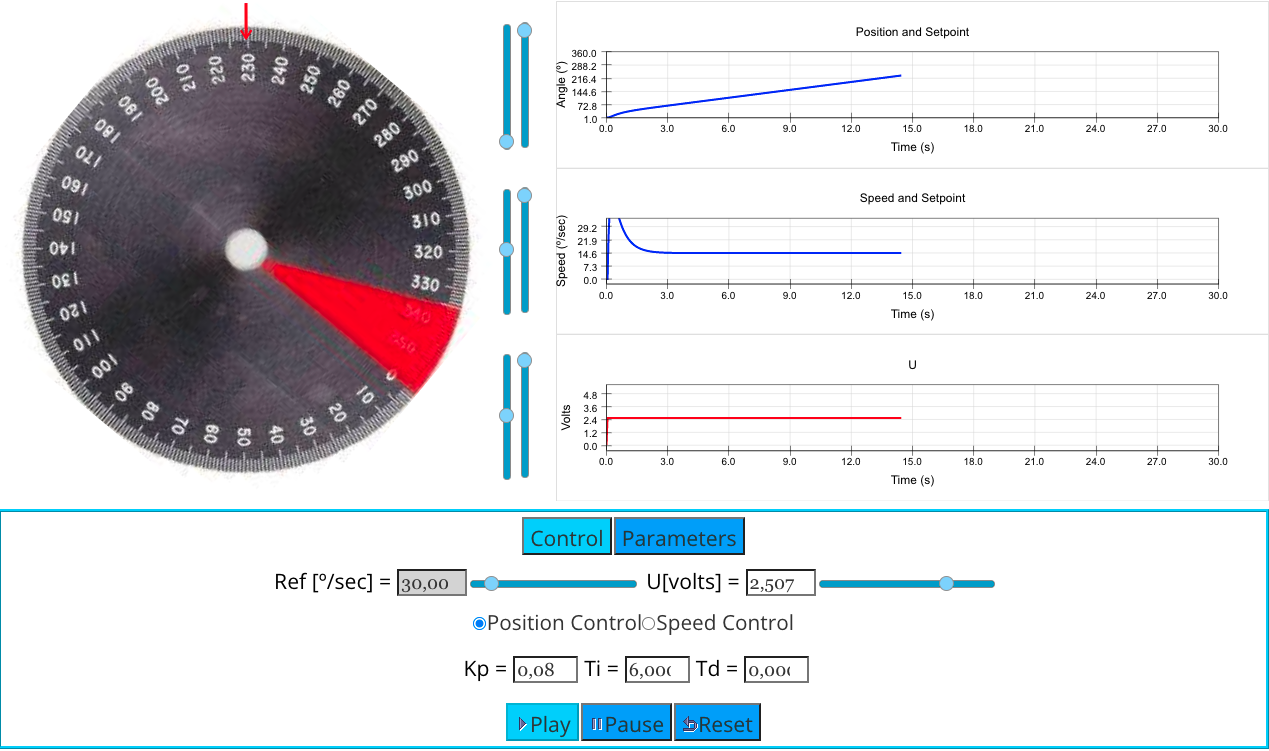
\includegraphics[scale = 0.35]{images/pt1-c-25-control.png}
\label{filtro1}
\caption{Medição a 2,5V - Controle}
\end{figure}

\begin{figure}[H]
\centering
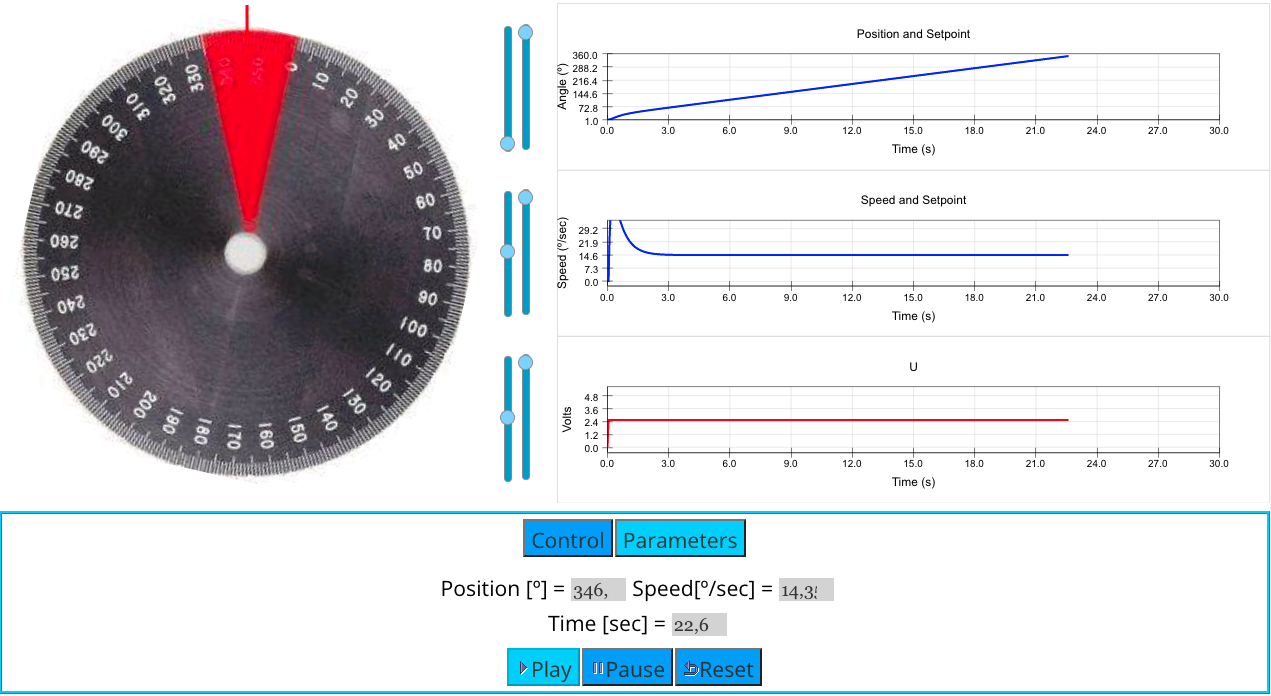
\includegraphics[scale = 0.35]{images/pt1-c-25-param.png}
\label{filtro1}
\caption{Medição a 2,5V - Parametros}
\end{figure}

Velocidade = 14,35º/sec\\\\

\newpage
- \qquad\qquad\> Para 3V: 
\begin{figure}[H]
\centering
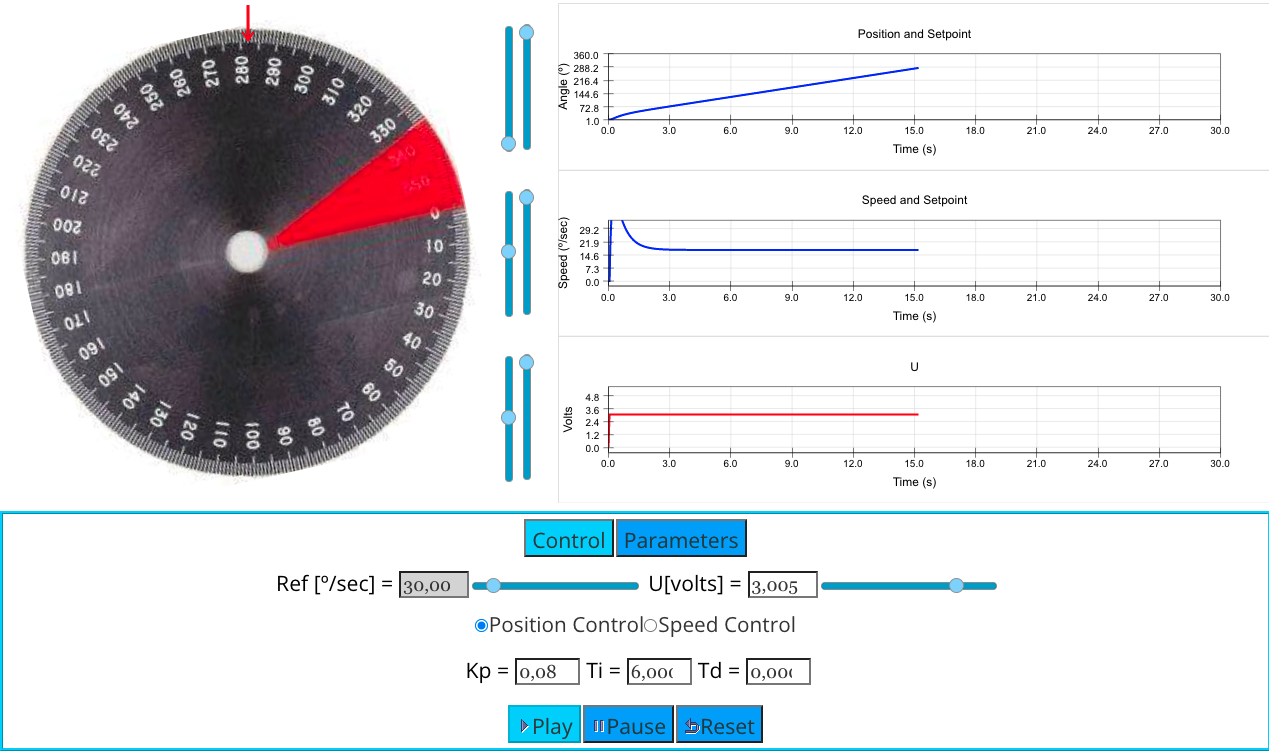
\includegraphics[scale = 0.35]{images/pt1-c-3-control.png}
\label{filtro1}
\caption{Medição a 3V - Controle}
\end{figure}

\begin{figure}[H]
\centering
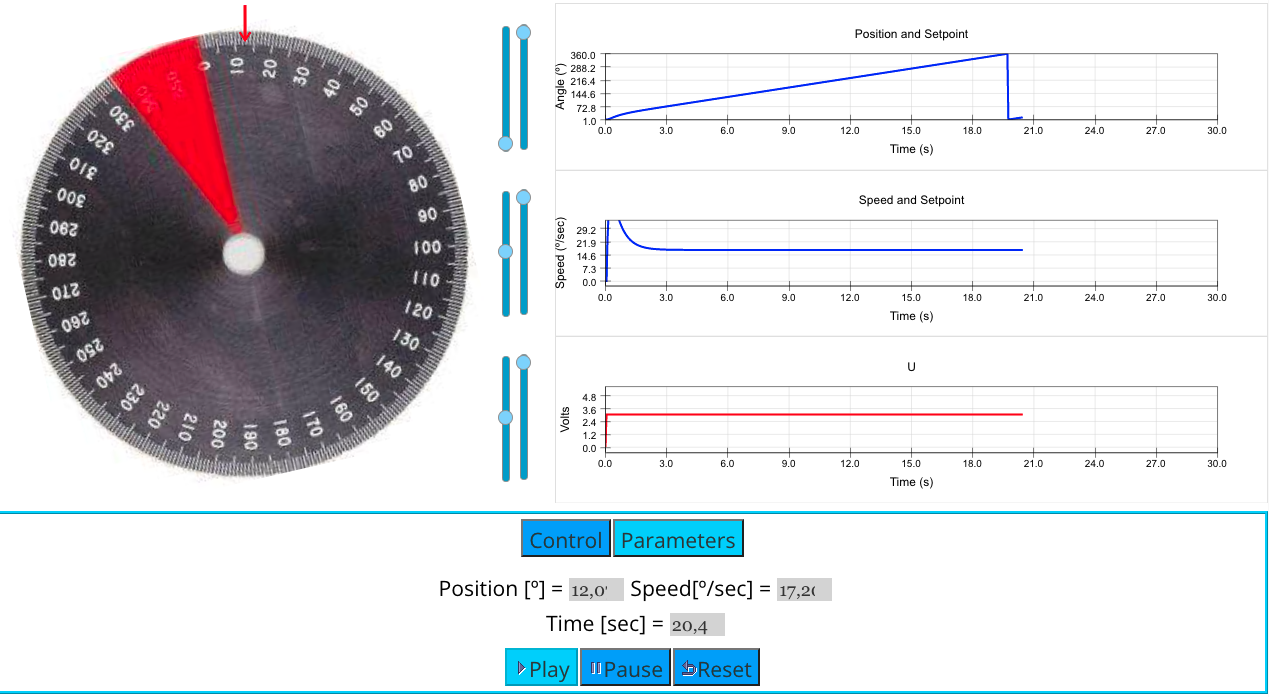
\includegraphics[scale = 0.35]{images/pt1-c-3-param.png}
\label{filtro1}
\caption{Medição a 3V - Parametros}
\end{figure}

Velocidade = 17,20º/sec\\\\


\paragraph{(d) Repita a seção (c) com valores de tensão de -1 V e -3V}:\\

Nota: O valor de $K_\omega$ obtido deve ser semelhante ao obtido no item anterior.

\newpage
- \qquad\qquad\> Para -1V: 
\begin{figure}[H]
\centering
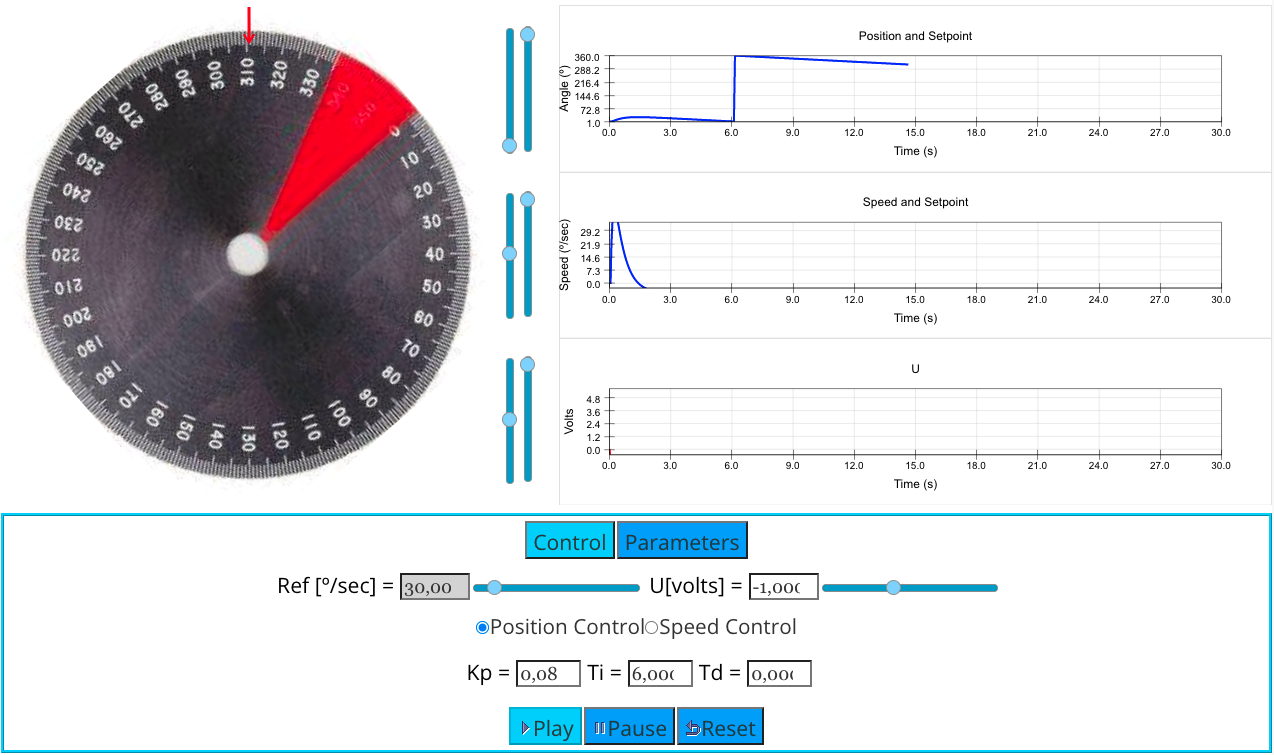
\includegraphics[scale = 0.35]{images/pt1-d-m1-control.png}
\label{filtro1}
\caption{Medição a -1V - Controle}
\end{figure}

\begin{figure}[H]
\centering
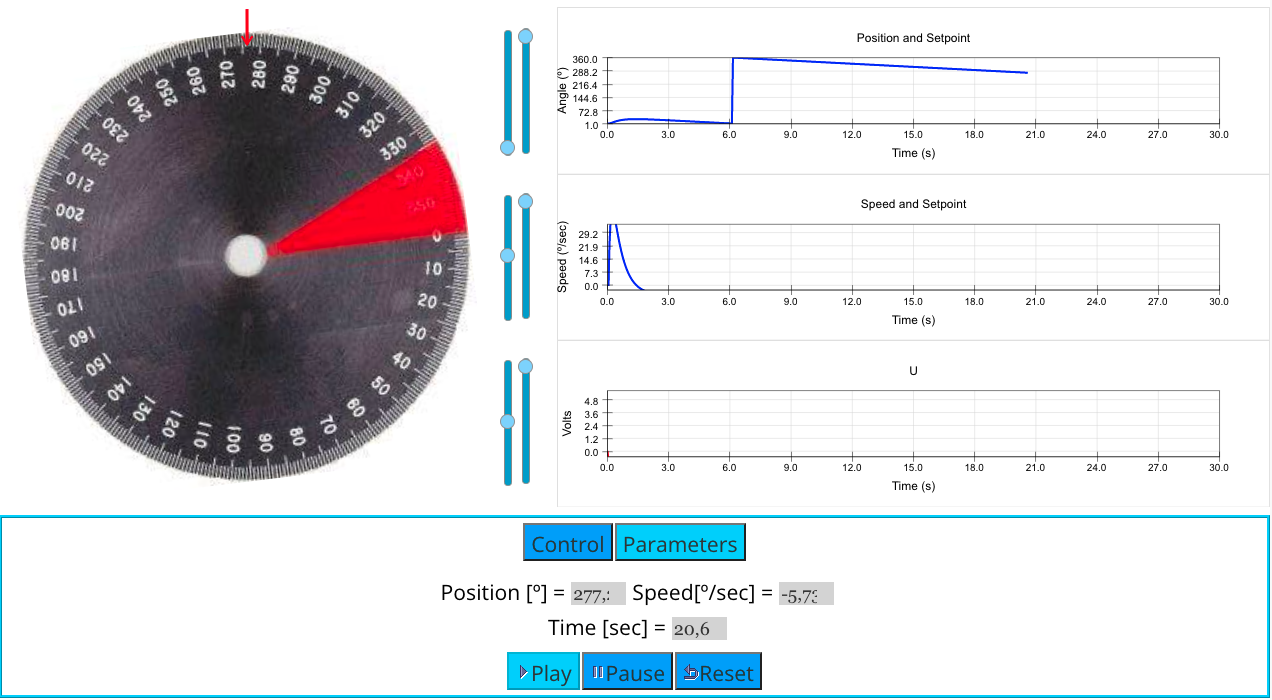
\includegraphics[scale = 0.35]{images/pt1-d-m1-param.png}
\label{filtro1}
\caption{Medição a -1V - Parametros}
\end{figure}

Velocidade = -5,73º/sec\\\\


\newpage
- \qquad\qquad\> Para -3V: 
\begin{figure}[H]
\centering
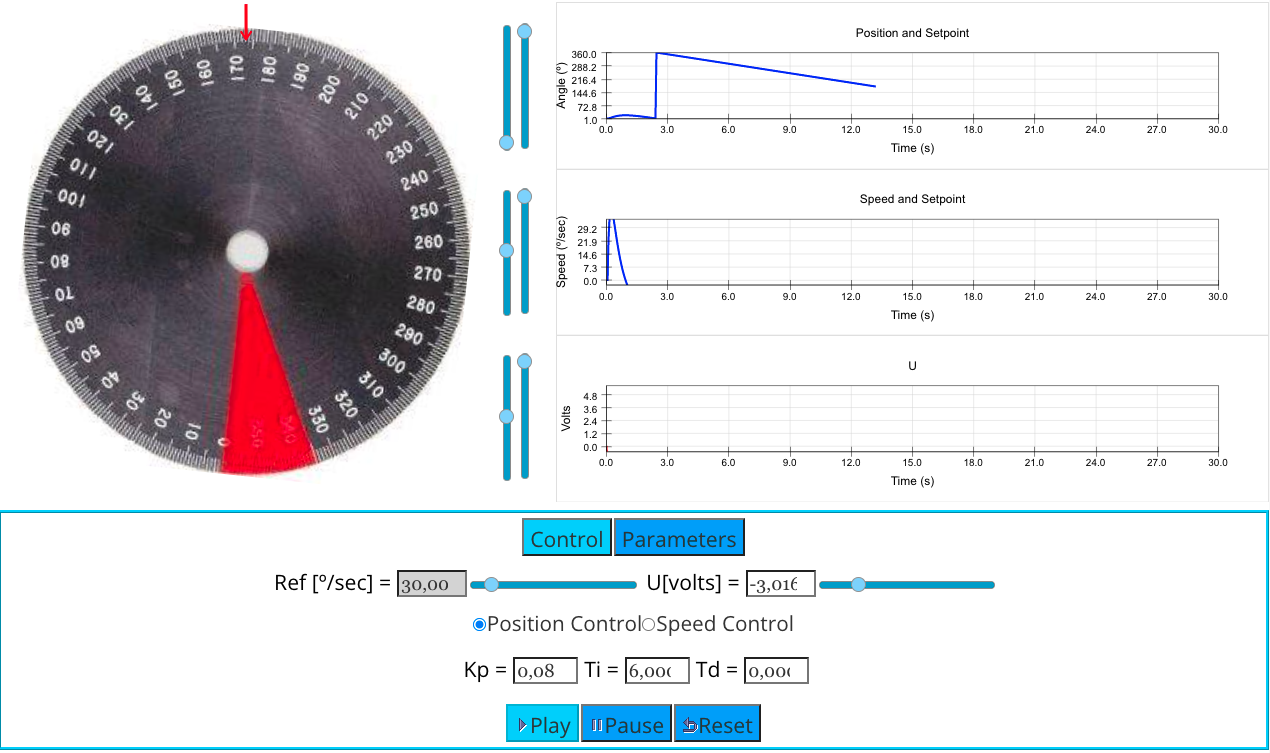
\includegraphics[scale = 0.35]{images/pt1-d-m3-control.png}
\label{filtro1}
\caption{Medição a -3V - Controle}
\end{figure}

\begin{figure}[H]
\centering
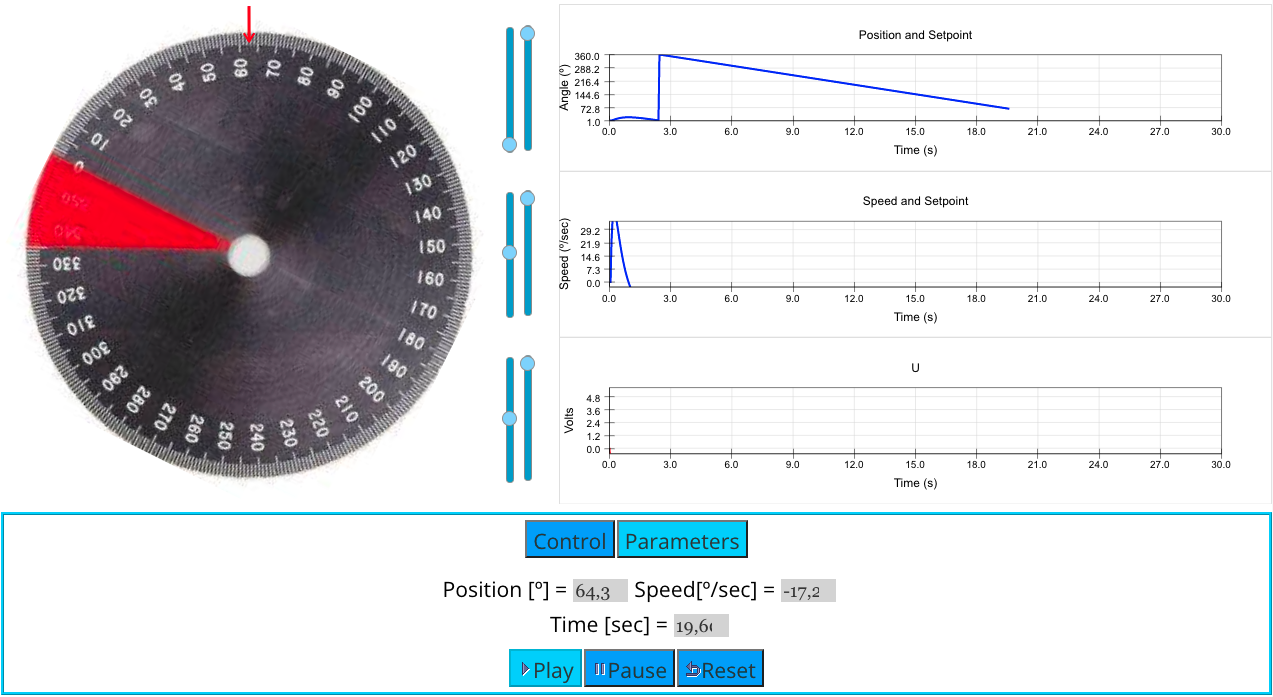
\includegraphics[scale = 0.35]{images/pt1-d-m3-param.png}
\label{filtro1}
\caption{Medição a -3V - Parametros}
\end{figure}

Velocidade = -17,2º/sec\\\\




\subsection{Tarefa 2 - Controle de Posição }
Utilizando o Laboratório Remoto da UNED (\url{https://unilabs.dia.uned.es/mod/ejsapp/view.php?
id=2417}), coloque o sistema em ângulo zero utilizando o “modo manual” e em seguida altere para “PID control”, ajuste para “position control” e faça os seguintes ensaios:\\

\textbf{a) Altere o ganho do controlador proporcional para os seguintes conjuntos de $Kp = [2, 0.5, 0.01]$ e zere os outros ganhos do controlador, em seguida troque o ângulo para 60º e verifique o que acontece, salve os gráficos de posição e velocidade e os compare, explicando se o acontecido faz sentido de acordo com o visualizado.}\\




\begin{figure}[H]
\centering
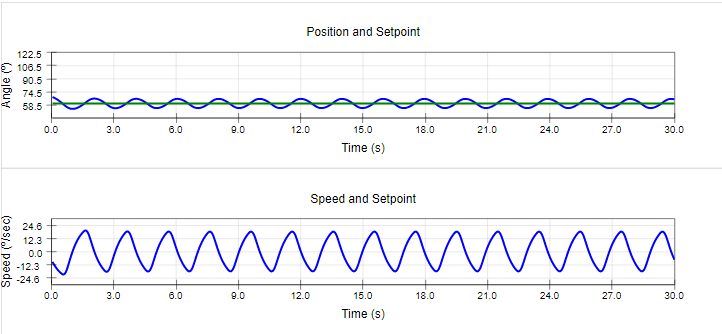
\includegraphics[scale = 0.8]{images/Tarefa_2_Kp_2.png}
\label{filtro1}
\caption{Kp = 2,00}
\end{figure}



\begin{figure}[H]
\centering
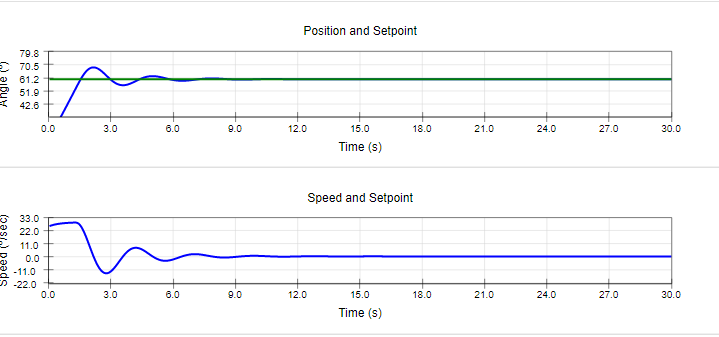
\includegraphics[scale = 0.8]{images/Tarefa_2_Kp_05.png}
\label{filtro1}
\caption{Kp = 0,5}
\end{figure}



\begin{figure}[H]
\centering
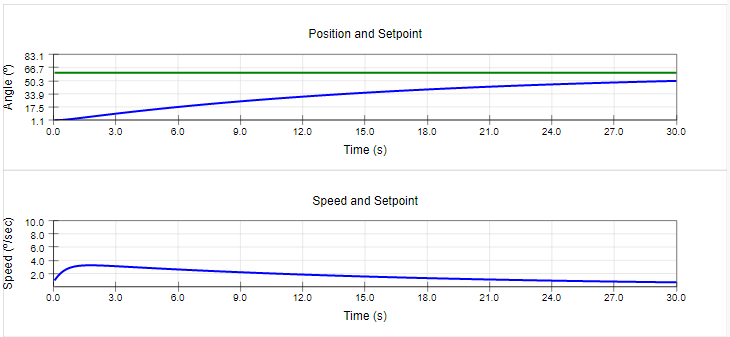
\includegraphics[scale = 0.8]{images/Tarefa_2_Kp_001.png}
\label{filtro1}
\caption{Kp = 0,01}
\end{figure}

Percebe-se que para um Kp igual a 2, o sistema é puramente oscilatório. Já com Kp igual a 0,5, o sistema apreseta um overshoot maior, porém se estabiliza com o tempo. Para Kp igual a 0,01, o sistema apresenta um maior tempo para estabilizar.\\




\textbf{(b) Repita o mesmo procedimento do item a, agora zerando os ganhos proporcional e derivativo e altere o ganho do controlador proporcional para os seguintes conjuntos de $T_i = [1, 0.5, 0.01]$. Verifique o que acontece, salve os gráficos de posição e velocidade com print e os compare, explicando se o acontecido faz sentido de acordo com o visualizado.}\\



\begin{figure}[H]
\centering
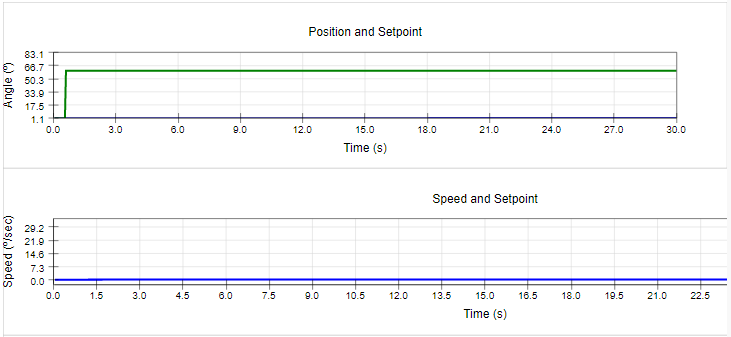
\includegraphics[scale = 0.8]{images/Tarefa_2_Ti_1.png}
\label{filtro1}
\caption{Ti = 1,0}
\end{figure}



\begin{figure}[H]
\centering
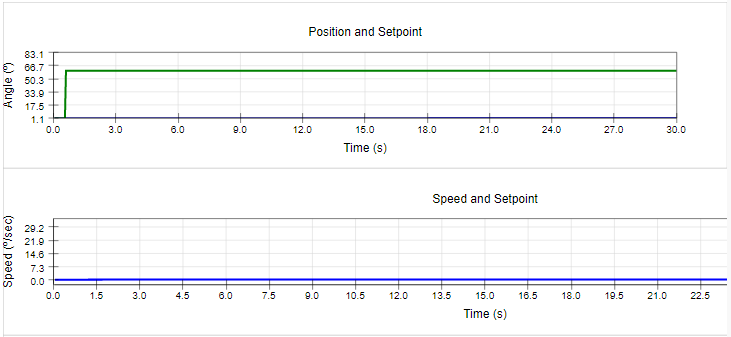
\includegraphics[scale = 0.8]{images/Tarefa_2_Ti_1.png}
\label{filtro1}
\caption{Ti = 0,5}
\end{figure}



\begin{figure}[H]
\centering
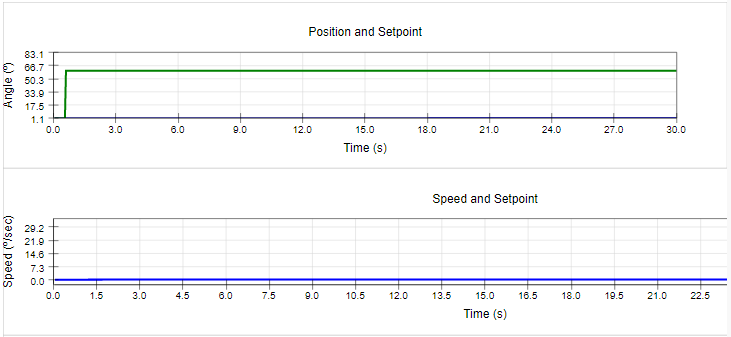
\includegraphics[scale = 0.8]{images/Tarefa_2_Ti_1.png}
\label{filtro1}
\caption{Ti = 0,01}
\end{figure}

Percebe-se que a resposta do sistema não altera com a variação de Ti enquanto os outros ganhos são iguais zero.\\

\textbf{(c) Repita o mesmo procedimento do item a, agora zerando o ganho derivativo e altere os ganhos dos controlador proporcional-integral para os seguintes conjuntos de $K_p = [1, 0.5, 0.08]$ e $T_i = [0.01, 1, 0.6]$. Verifique o que acontece, salve os gráficos de posição e velocidade com print e os compare, explicando se o acontecido faz sentido de acordo com o visualizado.}\\




\begin{figure}[H]
\centering
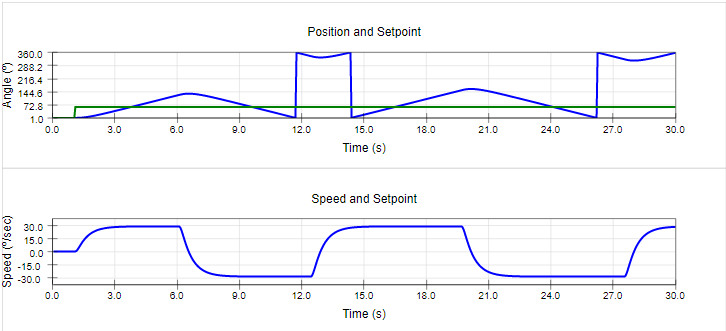
\includegraphics[scale = 0.8]{images/Tarefa_2_Kp_1_Ti_001_Td_1.png}
\label{filtro1}
\caption{Kp = 1 e Ti = 0,01}
\end{figure}



\begin{figure}[H]
\centering
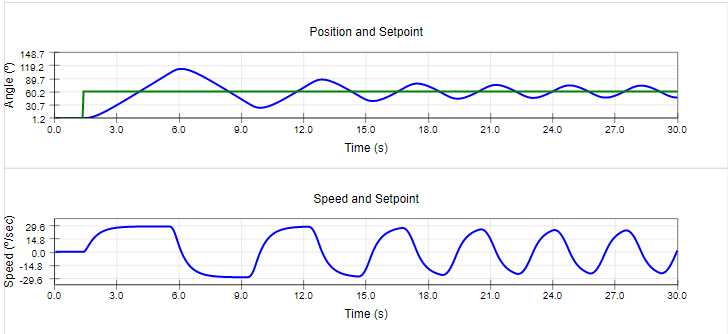
\includegraphics[scale = 0.8]{images/Tarefa_2_Kp_05_Ti_1.png}
\label{filtro1}
\caption{Kp = 0,5 e Ti = 1}
\end{figure}



\begin{figure}[H]
\centering
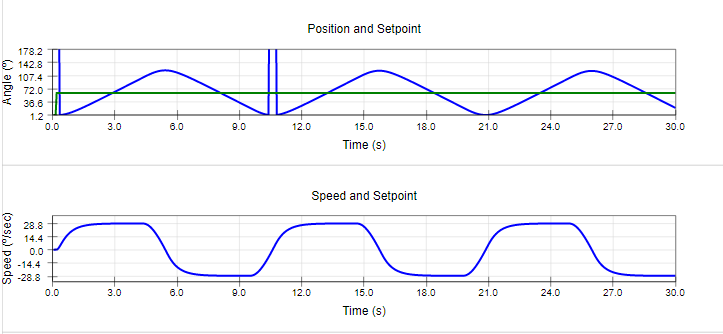
\includegraphics[scale = 0.8]{images/Tarefa_2_Kp_008_Ti_06.png}
\label{filtro1}
\caption{Kp = 0,08 e Ti = 0,6}
\end{figure}

Percebe-se que para os valores de Kp e Ti utilizados, o sistema se encontra como oscilatório, sendo então, insuficientes para estabilizá-lo.\\

\textbf{(d) Repita o mesmo procedimento do item a, alterando os ganhos do controlador proporcional-integral derivativo para os seguintes conjuntos de $K_p = [1, 0.5, 0.08]$, $T_i = [0.01, 1, 0.6]$ e $T_d = [1, 0.6, 0.01]$. Verifique o que acontece, salve os gráficos de posição e velocidade com print e os compare, explicando se o acontecido faz sentido de acordo com o visualizado.}\\





\begin{figure}[H]
\centering
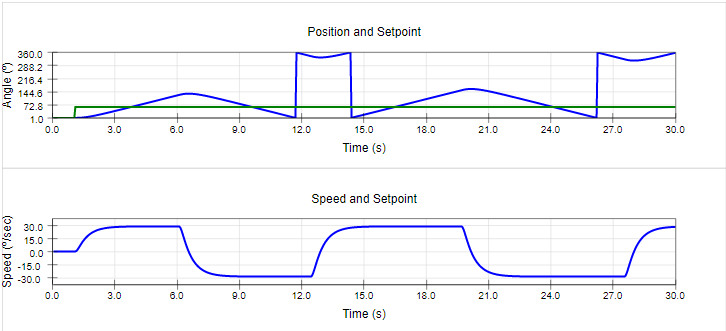
\includegraphics[scale = 0.8]{images/Tarefa_2_Kp_1_Ti_001_Td_1.png}
\label{filtro1}
\caption{Kp = 1, Ti = 0,01 e Td = 1}
\end{figure}



\begin{figure}[H]
\centering
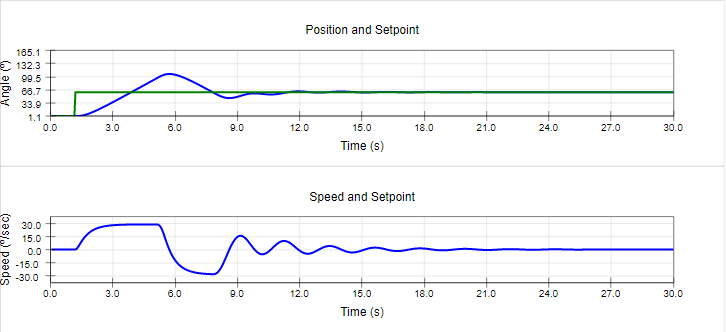
\includegraphics[scale = 0.8]{images/Tarefa_2_Kp_05_Ti_1_Td_06.png}
\label{filtroTI}
\caption{Kp = 0,5, Ti = 1 Td = 0,6}
\end{figure}



\begin{figure}[H]
\centering
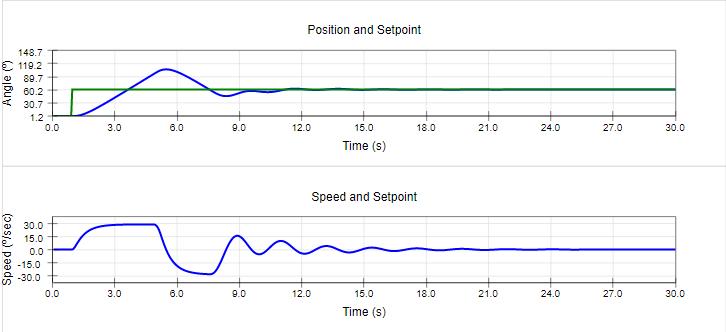
\includegraphics[scale = 0.8]{images/Tarefa_2_Kp_008_Ti_06_Td_001.png}
\label{filtro1PID}
\caption{Kp = 0,08, Ti = 0,6 e Td = 0,01}
\end{figure}

Com o controlador PID, percebe-se uma melhora na estabilidade do sistema de acordo com as Figuras 27 e 28, porém demonstram um tempo de assentamento maior.\\


\subsection{ Tarefa 3 - Controle de Velocidade}
Utilizando o laboratório remoto da UNED (\url{https://unilabs.dia.uned.es/mod/ejsapp/view.php?id=2417})
coloque o sistema em ângulo zero utilizando o “modo manual” e em seguida altere para “PID control”, ajuste para “speed control” e faça os seguintes ensaios:\\

\textbf{(a) Altere o ganho do controlador proporcional para os seguintes conjuntos de $K_p=[2, 0.5, 0.01]$ e zere os outros ganhos do controlador, em seguida troque o ângulo para 60º e verifique o que acontece, salve os gráficos de posição e velocidade com print e os compare, explicando se o acontecido faz sentido de acordo com o visualizado.}\\

\begin{figure}[H]
\centering
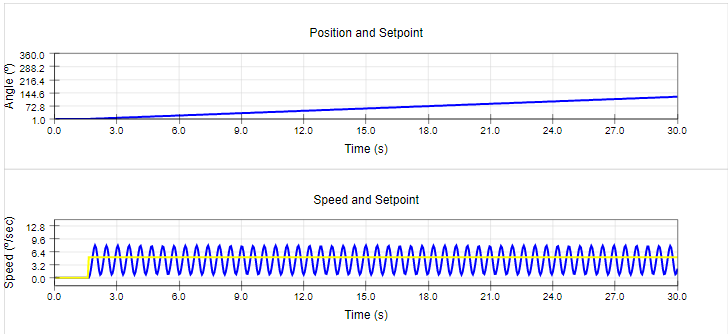
\includegraphics[scale = 0.8]{images/Tarefa_3_Kp_2.png}
\label{filtro1}
\caption{Kp = 2,00}
\end{figure}



\begin{figure}[H]
\centering
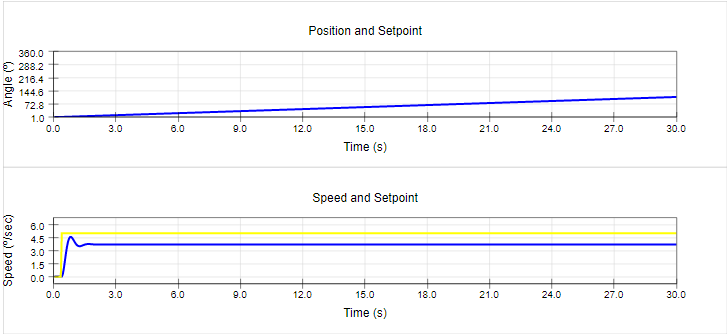
\includegraphics[scale = 0.8]{images/Tarefa_3_Kp_05.png}
\label{filtro1}
\caption{Kp = 0,5}
\end{figure}



\begin{figure}[H]
\centering
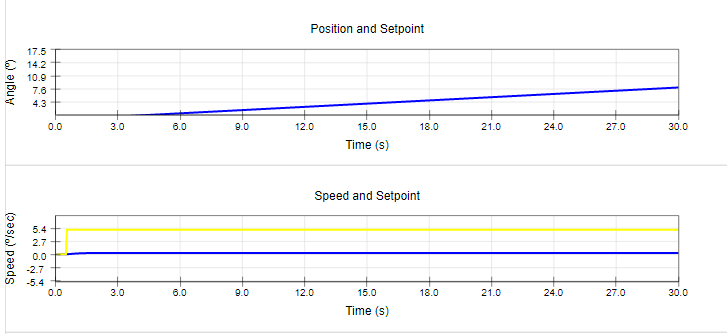
\includegraphics[scale = 0.8]{images/Tarefa_3_Kp_001.png}
\label{filtro1}
\caption{Kp = 0,01}
\end{figure}

Para o controle da velocidade, o sistema é oscilatório para Kp igual 2, se estabiliza lentamente com Kp igual a 0,5.\\

\textbf{(b) Repita o mesmo procedimento do item a, agora zerando os ganhos proporcional e derivativo e altere o ganho do controlador proporcional para os seguintes conjuntos de $T_i=[1, 0.5, 0.01]$. Verifique o que
acontece, salve os gráficos de posição e velocidade com print e os compare, explicando se o acontecido faz sentido de acordo com o visualizado.}\\

\begin{figure}[H]
\centering
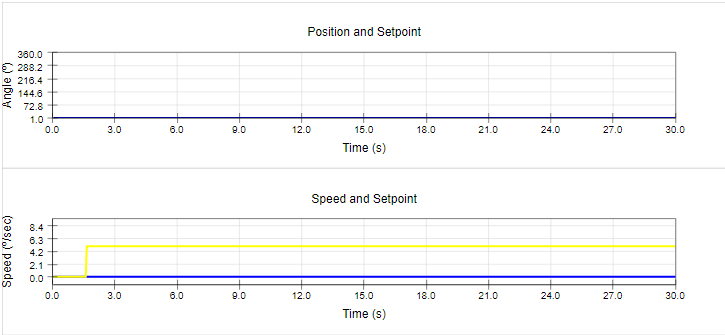
\includegraphics[scale = 0.8]{images/Tarefa_3_Ti_1_05_001.png}
\label{filtro1}
\caption{Ti = 1,0}
\end{figure}



\begin{figure}[H]
\centering
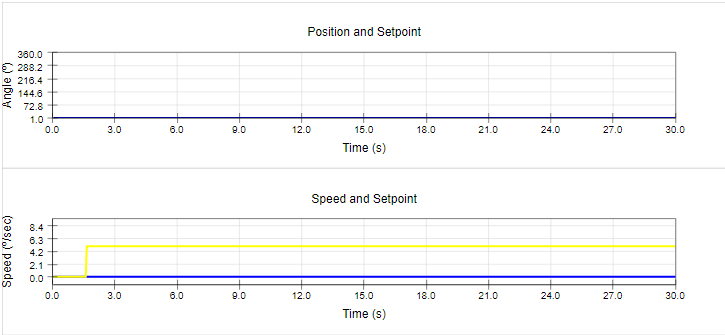
\includegraphics[scale = 0.8]{images/Tarefa_3_Ti_1_05_001.png}
\label{filtro1}
\caption{Ti = 0,5}
\end{figure}



\begin{figure}[H]
\centering
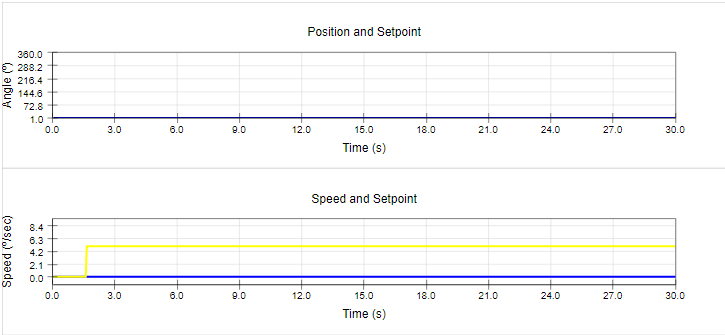
\includegraphics[scale = 0.8]{images/Tarefa_3_Ti_1_05_001.png}
\label{filtro1}
\caption{Ti = 0,01}
\end{figure}

Percebe-se que para os valores de Kp e Ti utilizados, o sistema se encontra como oscilatório, sendo então, insuficientes para estabilizá-lo.\\

\textbf{(c) Repita o mesmo procedimento do item a, agora zerando o ganho derivativo e altere os ganhos dos controlador proporcional-integral para os seguintes conjuntos de Kp=[1, 0.5, 0.08] e Ti=[0.01, 1, 0.6]. Verifique o que acontece, salve os gráficos de posição e velocidade com print e os compare, explicando se o acontecido faz sentido de acordo com o visualizado.}\\

\begin{figure}[H]
\centering
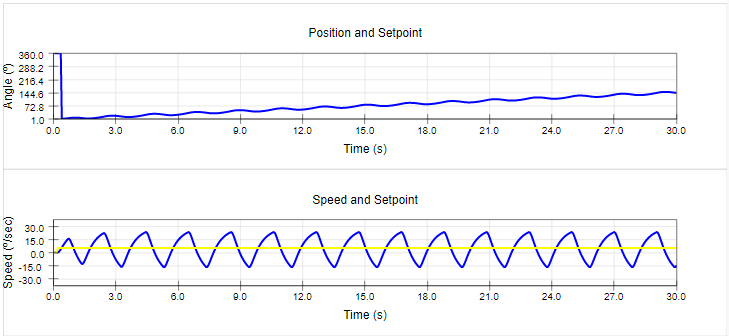
\includegraphics[scale = 0.8]{images/Tarefa_3_Kp_1_Ti_001_Td_1.png}
\label{filtro1KPTI}
\caption{Kp = 1 e Ti = 0,01}
\end{figure}



\begin{figure}[H]
\centering
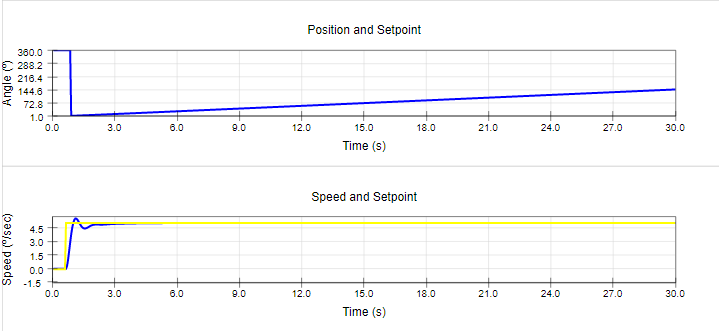
\includegraphics[scale = 0.8]{images/Tarefa_3_Kp_05_Ti_1.png}
\label{filtro1KPTI2}
\caption{Kp = 0,5 e Ti = 1}
\end{figure}



\begin{figure}[H]
\centering
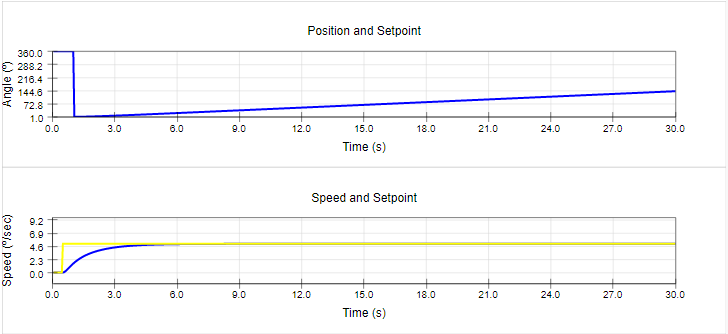
\includegraphics[scale = 0.8]{images/Tarefa_3_Kp_008_Ti_06.png}
\label{filtro1KPTI3}
\caption{Kp = 0,08 e Ti = 0,6}
\end{figure}

Percebe-se na Figura 35 que o sistema é oscilatório. Na Figura 36, o sistema estabiliza, porém com um overshoot elevado. Já na Figura 37, o sistema possui um tempo de assentamento maior, porém estabiliza.\\




\textbf{(d) Repita o mesmo procedimento do item a, alterando os ganhos do controlador proporcional-integralderivativo para os seguintes conjuntos de $K_p=[1, 0.5, 0.08]$, $T_i=[0.01, 1, 0.6]$ e $T_d=[1, 0.6, 0.01]$. Verifique o que acontece, salve os gráficos de posição e velocidade com print e os compare, explicando se o acontecido faz sentido de acordo com o visualizado.}\\

\begin{figure}[H]
\centering
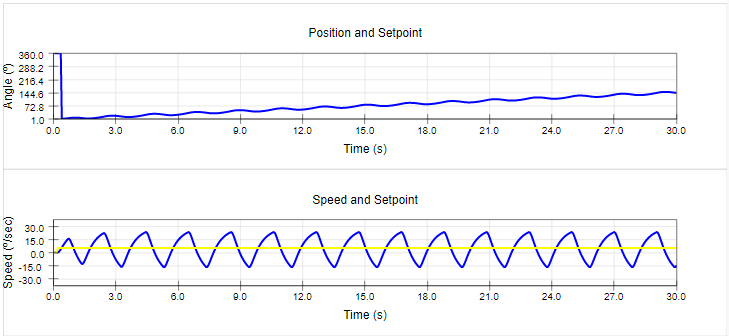
\includegraphics[scale = 0.8]{images/Tarefa_3_Kp_1_Ti_001_Td_1.png}
\label{filtro1PID}
\caption{Kp = 1, Ti = 0,01 e Td = 1}
\end{figure}



\begin{figure}[H]
\centering
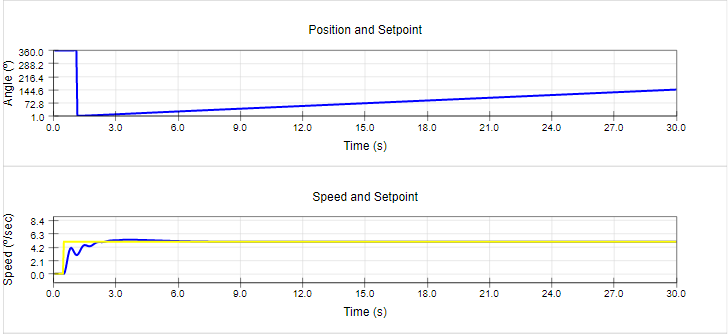
\includegraphics[scale = 0.8]{images/Tarefa_3_Kp_05_Ti_1_Td_06.png}
\label{filtro1PID2}
\caption{Kp = 0,5, Ti = 1 Td = 0,6}
\end{figure}



\begin{figure}[H]
\centering
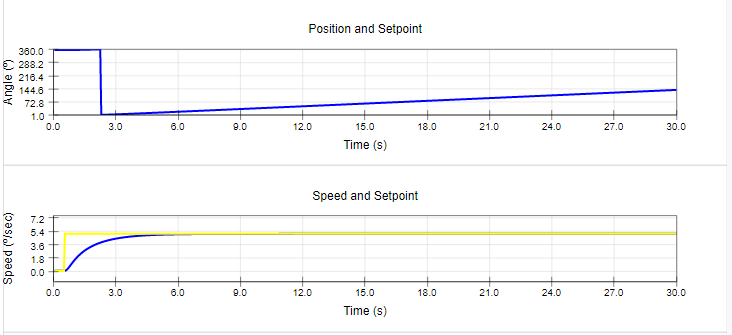
\includegraphics[scale = 0.8]{images/Tarefa_3_Kp_008_Ti_06_Td_001.png}
\label{filtro1PID3}
\caption{Kp = 0,08, Ti = 0,6 e Td = 0,01}
\end{figure}


Com o controlador PID, o sistema ainda permanece oscilatório para as constantes na Figura 38, porém ao alterar as constantes gerando a Figura 39, o sistema estabiliza com leves oscilações. Já na Figura 40, o sistema não apresenta overshoot, estabiliza mas tem tempo de assentamento maior.\\


\newpage

% REFERENCIAS %%%%%%%%%%%%%%%%%%%%%%%%%%%%%%%%%%%%%%%%%%%%%%%%%%%%%%%%%%%%%%
    \nocite{*}
    \bibliography{src/bibliography}
    
\end{document}
\section{Referências Bibliográficas}

\end{document}